\documentclass{beamer}
\usetheme{Madrid}
% \usetheme{default}
% \usecolortheme{beaver}
\usepackage{graphicx}
\graphicspath{ {pics} }
\usepackage{amsmath}
\usepackage{amssymb}
\usepackage{framed}
\usepackage{tikz}
\setbeamercolor{mycolorbox}{%
  bg=blue!20,   % background color (20% blue)
  fg=black      % foreground (text) color
}
\usefonttheme[onlymath]{serif}

%Information to be included in the title page:
\title{Algebra}
\author{Nithin}
\institute{Maveric Systems}
\date{\today}

\begin{document}
\frame{\titlepage}
\section{Introduction}
\begin{frame}{Origins of Algebra}
    \begin{itemize}
      \item \textbf{Mesopotamia \& Egypt (c. 2000–1600 BCE)}
        \begin{itemize}
          \item Early problem-solving (linear/quadratic equations) in word problems
          \item No formal symbols, but systematic procedures
        \end{itemize}
  
      \item \textbf{Greek Era (c. 600 BCE–300 CE)}
        \begin{itemize}
          \item Geometric methods for solving equations (Euclid, Apollonius)
          \item Diophantus introduced proto-symbolic notation
        \end{itemize}
  
      \item \textbf{Islamic Golden Age (8th–12th Century)}
        \begin{itemize}
          \item Al-Khwarizmi’s work \emph{Al-jabr} $\rightarrow$ term “Algebra”
          \item Systematic solutions for linear and quadratic equations
        \end{itemize}
  
      \item \textbf{Transmission to Europe (12th–17th Century)}
        \begin{itemize}
          \item Latin translations influenced Fibonacci, others
          \item Viète, Descartes established modern symbolic notation \& analytic geometry
        \end{itemize}
  
      \item \textbf{Modern Algebra (19th–20th Century)}
        \begin{itemize}
          \item Emergence of abstract algebra (groups, rings, fields)
          \item Galois, Abel, and others formalized algebraic structures
        \end{itemize}
    \end{itemize}
  \end{frame}
  \begin{frame}{What is Algebra?}
    Algebra is a branch of mathematics that deals with numbers, variables, and their relationships. Key concepts include:
    \begin{itemize}
        \item \textbf{Variables}: Symbols (like \( x \), \( y \)) representing unknown or changing values.
        \item \textbf{Expressions}: Combinations of variables, numbers, and operations. E.g., \( 2x + 3 \).
        \item \textbf{Equations}: Mathematical statements that express equality, e.g., \( 2x + 3 = 7 \).
        \item \textbf{Solving Equations}: Finding values for variables that make an equation true.
        \item \textbf{Polynomials}: Expressions like \( 3x^2 + 2x - 5 \) involving variables raised to powers.
        \item \textbf{Functions}: Describes a relationship between variables, e.g., \( y = 2x + 1 \).
    \end{itemize}
\end{frame}
  \begin{frame}{Integers}
    \begin{itemize}
        \item The set of integers is denoted by \(\mathbb{Z}\).
        \item Integers include:
        \[
          \ldots, -3, -2, -1, 0, 1, 2, 3, \ldots
        \]
        \item Formally, \(\mathbb{Z} = \{\dots, -2, -1, 0, 1, 2, \dots\}\).
        \item Common properties:
        \begin{itemize}
            \item \(\mathbb{Z}\) is infinite and unbounded in both the negative and positive directions.
            \item Closed under addition, subtraction, and multiplication:
                \[
                  \forall a, b \in \mathbb{Z}, \quad
                  a \pm b \in \mathbb{Z}, \quad
                  a \cdot b \in \mathbb{Z}.
                \]
        \end{itemize}
        \item The quotient of any two integers is not necessarily an integer. So we need to extend arithmetic to \textbf{rational numbers}
    \end{itemize}
\end{frame}
% Slide: Rational Numbers
\begin{frame}{Rational Numbers}
    \begin{itemize}
        \item The set of rational numbers is denoted by \(\mathbb{Q}\).
        \item Definition:
        \[
          \mathbb{Q} = \left\{ \frac{p}{q} \,\middle|\,
            p \in \mathbb{Z}, \; q \in \mathbb{Z}, \; q \neq 0
          \right\}.
        \]
        \item Every integer is also a rational number (e.g., \(5 = \frac{5}{1}\)).
        \item Examples:
        \[
          \frac{1}{2}, \quad -\frac{3}{4}, \quad 0, \quad 7, \quad \frac{11}{5}, \ldots
        \]
        \item Properties:
        \begin{itemize}
            \item Closed under addition, subtraction, multiplication, and division (except division by zero).
            \item Densely packed on the number line: between any two rationals, there is another rational.
        \end{itemize}
    \end{itemize}
\end{frame}
\begin{frame}
    \frametitle{Interesting Facts}
    \begin{itemize} 
        \item Why division by zero is prohibited ?
        \begin{itemize}
            \item Division is inverse of multiplication in the sense  
            \[  
            \frac{m}{n} \cdot n = m
            \]
        \item if \( n=0 \) and \( m = 1\), we get \(\frac{1}{0} \cdot 0 = 1\) which is nonsensical as any number multiplied by zero is zero
        \end{itemize}
        \item Rational numbers suffice for all actual physical measurements like weight, height and length
        \item But Geometry, Algebra and Calculus force us to consider \textbf{real numbers}
    \end{itemize}
\end{frame}
\begin{frame}
    \frametitle{A Real Number Line}
    \begin{figure}[h]    
        \begin{minipage}[b]{0.8\textwidth}
        \centering
        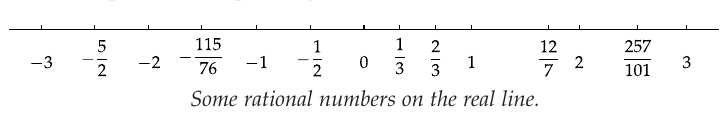
\includegraphics[scale=0.35]{real-line.png}
    \end{minipage}
\end{figure}
\begin{itemize}
    \item if \( n\) is a positive integer then \( \frac{1}{n}\) is to the right of 0 by the length obtained by dividing the segment from \( 1 to 0\) in to \( n \) segments of equal length
\end{itemize}
\end{frame}
\begin{frame}
    \frametitle{Is every Real Number a Rational}
    \begin{figure}[h]    
        \begin{minipage}[b]{0.8\textwidth}
        \centering
        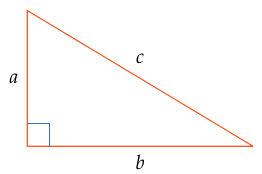
\includegraphics[scale=0.35]{irrational-geometry.png}
        \end{minipage}
    \end{figure}
    \begin{itemize}
        \item \( c^{2} = a^{2} + b^{2} \). If \( a = 1, b = 1\) then \(c^{2} = 2 \). Then what rational number is \( c \)
        \item By trial and error, \( c = \left( \frac{99}{70} \right)^{2}  = \frac{9801}{4900}\) where the numerator just misses twice the denominator by 1. But this is not 2 but close to 2. Another number is \( \left( \frac{9369319}{6625109} \right)^{2} = 1.999999999999977\) , but not 2
        \item Greeks proved that it is impossible to find any rational number whose square is 2
    \end{itemize} 
\end{frame}
\begin{frame}
    \frametitle{Proof: No rational number has a square equal to 2}
    Let m and n are two integers
    \[ 
        \left( \frac{m}{n} \right)^{2} = 2  
    \]
    By canceling any common factors, m and n are reduces to its lowest terms 

    \[
         m^{2} = 2n^{2}
    \]

    this makes \(m^{2}\) even, hence \(m\) is an even. (The square of even is even and odd is odd). So \(m = 2k\) for some integer \(k\)

    Substituting \(m = 2k\) in the equation gives, \(4k^{2} = 2n^{2} \), which results in 
    \[
        2k^{2} = n^{2}
    \]
    which means \( n^{2}\) is even and therefore \(n \) is even
    \\
    \(\frac{m}{n} \) has common factors which contradicts the earlier assumption
\end{frame}
\begin{frame}
    \frametitle{Irrational Number}

    \begin{block}{Irrational Number}
        A real number that is not rational is \textbf{irrational number}
    \end{block}
    \begin{itemize}
        \item \( \sqrt(2)\)
        \item \(3+\sqrt(2)\)
        \item \(8\sqrt(2)\)
    \end{itemize}
\end{frame}
\section{Algebra of real numbers}
\begin{frame}{Properties of Real Numbers}
  \begin{itemize}
      \item \textbf{Commutative Properties}
      \begin{itemize}
          \item Addition: $a + b = b + a$
          \item Multiplication: $a \cdot b = b \cdot a$
      \end{itemize}
      \vspace{5pt}

      \item \textbf{Associative Properties}
      \begin{itemize}
          \item Addition: $(a + b) + c = a + (b + c)$
          \item Multiplication: $(a \cdot b) \cdot c = a \cdot (b \cdot c)$
      \end{itemize}
      \vspace{5pt}
      \item \textbf{Distributive Property}
      \begin{itemize}
          \item $a \cdot (b + c) = (a \cdot b) + (a \cdot c)$
      \end{itemize}
      \vspace{5pt}
      \item \textbf{Identity Elements}
      \begin{itemize}
          \item Additive Identity: $a + 0 = a$
          \item Multiplicative Identity: $a \cdot 1 = a$
      \end{itemize}
      \vspace{5pt}
      \item \textbf{Inverse Elements}
      \begin{itemize}
          \item Additive Inverse: $a + (-a) = 0$
          \item Multiplicative Inverse (if $a \neq 0$): $a \cdot \frac{1}{a} = 1$
      \end{itemize}
    \end{itemize}
    \end{frame}
    \begin{frame}{Properties of Real Numbers}
    \begin{itemize}
      \vspace{5pt}
      \item \textbf{Closure Property}
      \begin{itemize}
          \item Real numbers are closed under addition, subtraction, multiplication, and division (except division by zero).
      \end{itemize}
  \end{itemize}
  \end{frame}
\subsection{Inequalities,Intervals and Absolute Value}
\begin{frame}
  \frametitle{Inequalities}
  \begin{block}{Transitivity}
    \begin{itemize}
        \item If $a < b$ and $b < c$, then $a < c$
      \end{itemize}
  \end{block}
  \begin{block}{Multiplication}
    Suppose $a < b$
    \begin{itemize}
      \item If $c > 0$, then $ac < bc$
      \item If $c <  0$, then $ ac > bc$
    \end{itemize}
  \end{block}
\end{frame} 
\begin{frame}
  \frametitle{Exercise }
  Find all number \( x \) such that 
  \[\frac{x-8}{x-4} < 3 \] 
Our first step  is to multiply by \(x-4\)
Here there are two conditions:
\begin{enumerate}
  \item \( x-4 > 0 \) 
  \[ x -8 < 3(x-4)  \implies x-8 < 3x-12 \implies 2x > 4  \implies x > 2\]
  But our initial assumption is \(x-4 > 0 \implies x > 4 \). As \( 4 > 2 \), original inequality holds if \( x > 4\)
\end{enumerate} 
\end{frame}
\begin{frame}
  \frametitle{Exercise Conti.}
\begin{enumerate}
  \setcounter{enumi}{1}
  \item \( x-4 < 0 \) 
  \[ x-8 > 3(x-4) \implies  x < 2 \] 
  Initial assumption is \( x<4 \). As \( 2 < 4\), inequality holds for \( x < 2 \)
\end{enumerate}
The original inequality holds true for \[x < 2 ,  x > 4 \]   
or 
\[  (-\infty, 2) \cup (4,\infty) \]
\end{frame}
\begin{frame}
  \frametitle{Inequalities}
  \begin{block}{Additive Inverse}
    If \( a < b \) then \( -a > -b \)
    Direction of inequalities has to be reversed when taking additive inverses on both sides 
  \end{block}
  \begin{block}{Multiplicative Inverse}
    If \( a < b \) 
    \begin{itemize}
      \item If \(a > 0, b > 0\), then \(\frac{1}{a} > \frac{1}{b} \)
      \item If \(a < 0 < b\), then \(\frac{1}{a} < \frac{1}{b} \)
    \end{itemize} 
  \end{block}
\end{frame}
\begin{frame}{What is a Set?}
  \begin{block}{Definition}
      A \textbf{set} is a well-defined collection of distinct objects, called \textbf{elements} or \textbf{members} of the set.
  \end{block}
  \vspace{10pt}
  \textbf{Representation of a Set:}
  \begin{itemize}
      \item \textbf{Roster Form:} List elements inside curly braces:
      \[
      A = \{1, 2, 3, 4\}
      \]
      \item \textbf{Set-Builder Notation:} Describe properties of elements:
      \[
      A = \{x \mid x \text{ is a positive integer less than 5}\}
      \]
  \end{itemize}
  \vspace{10pt}
  \begin{block}{Membership}
      \begin{itemize}
          \item If \(x\) belongs to \(A\), write \(x \in A\).
          \item If \(x\) does not belong to \(A\), write \(x \notin A\).
      \end{itemize}
  \end{block}
\end{frame}
\begin{frame}{Types of Sets}
  \begin{block}{Types of Sets}
      \begin{itemize}
          \item \textbf{Finite Set:} A set with a countable number of elements. \\
          Example: \(A = \{1, 2, 3, 4\}\)
          
          \item \textbf{Infinite Set:} A set with an uncountable or infinite number of elements. \\
          Example: \(\mathbb{N} = \{1, 2, 3, \dots\}\)

          \item \textbf{Empty/Null Set:} A set with no elements, denoted as \(\emptyset\) or \(\{\}\).

          \item \textbf{Subset:} \(A \subseteq B\) if every element of \(A\) is in \(B\).

          \item \textbf{Universal Set:} A set containing all objects under consideration, usually denoted by \(U\).

          \item \textbf{Power Set:} The set of all subsets of \(A\), denoted as \(P(A)\). \\
          Example: If \(A = \{1, 2\}\), then \(P(A) = \{\emptyset, \{1\}, \{2\}, \{1, 2\}\}\).
      \end{itemize}
  \end{block}
\end{frame}
\begin{frame}{Set Operations}
  \begin{block}{Union (\(\cup\))}
      Combines elements of two sets:
      \[
      A \cup B = \{x \mid x \in A \text{ or } x \in B\}
      \]
  \end{block}
  \begin{block}{Intersection (\(\cap\))}
      Elements common to both sets:
      \[
      A \cap B = \{x \mid x \in A \text{ and } x \in B\}
      \]
  \end{block}
  \begin{block}{Difference (\(A - B\))}
      Elements in \(A\) but not in \(B\):
      \[
      A - B = \{x \mid x \in A \text{ and } x \notin B\}
      \]
  \end{block}
\end{frame}
\begin{frame}{Set Operations}
  \begin{block}{Complement (\(A^c\))}
    Elements not in the set \(A\):
    \[
    A^c = \{x \mid x \notin A\}
    \]
\end{block}
  \begin{block}{Examples}
      \begin{itemize}
          \item The set of natural numbers: \(\mathbb{N} = \{1, 2, 3, \dots\}\).
          \item The set of integers: \(\mathbb{Z} = \{\dots, -3, -2, -1, 0, 1, 2, 3, \dots\}\).
          \item The set of even numbers: \(\{2, 4, 6, \dots\}\).
      \end{itemize}
  \end{block}
\end{frame} 
\begin{frame}{What is an Interval?}
  \begin{block}{Definition}
      An \textbf{interval} is a set of real numbers that includes all the numbers between two given endpoints.
  \end{block}
  \vspace{10pt}
  Intervals describe ranges of values on the real number line and are widely used in mathematics.
\end{frame}
% Slide 3: Types of Intervals
\begin{frame}{Types of Intervals}
  \begin{itemize}
      \item \textbf{Closed Interval (\([a, b]\))}: Includes both endpoints \(a\) and \(b\).
      \[
      [a, b] = \{x \in \mathbb{R} \mid a \leq x \leq b\}
      \]
      Example: \([2, 5] = \{x \mid 2 \leq x \leq 5\}\).
      \vspace{5pt}

      \item \textbf{Open Interval (\((a, b)\))}: Excludes both endpoints \(a\) and \(b\).
      \[
      (a, b) = \{x \in \mathbb{R} \mid a < x < b\}
      \]
      Example: \((2, 5) = \{x \mid 2 < x < 5\}\).
  \end{itemize}
\end{frame}
% Slide 4: Half-Open Intervals
\begin{frame}{Half-Open or Half-Closed Intervals}
  \begin{itemize}
      \item \textbf{Left-Closed, Right-Open (\([a, b)\))}:
      \[
      [a, b) = \{x \in \mathbb{R} \mid a \leq x < b\}
      \]
      Example: \([2, 5) = \{x \mid 2 \leq x < 5\}\).
      \vspace{5pt}

      \item \textbf{Left-Open, Right-Closed (\((a, b]\))}:
      \[
      (a, b] = \{x \in \mathbb{R} \mid a < x \leq b\}
      \]
      Example: \((2, 5] = \{x \mid 2 < x \leq 5\}\).
  \end{itemize}
\end{frame}
% Slide 5: Infinite Intervals
\begin{frame}{Infinite Intervals}
  \begin{itemize}
      \item \((a, \infty)\): All numbers greater than \(a\).
      \[
      (a, \infty) = \{x \in \mathbb{R} \mid x > a\}
      \]
      Example: \((3, \infty)\) includes all numbers greater than 3.

      \item \((-\infty, b)\): All numbers less than \(b\).
      \[
      (-\infty, b) = \{x \in \mathbb{R} \mid x < b\}
      \]
      Example: \((-\infty, 4)\) includes all numbers less than 4.

      \item \((-\infty, \infty)\): The entire real number line.
      \[
      (-\infty, \infty) = \mathbb{R}
      \]
  \end{itemize}
\end{frame}
% Slide 6: Summary Table
\begin{frame}{Summary of Interval Types}
  \begin{tabular}{|c|c|c|}
      \hline
      \textbf{Type} & \textbf{Interval Notation} & \textbf{Description} \\
      \hline
      Closed         & \([a, b]\)      & Includes both endpoints \(a, b\) \\
      Open           & \((a, b)\)      & Excludes both endpoints \(a, b\) \\
      Half-Open Left & \([a, b)\)      & Includes \(a\), excludes \(b\) \\
      Half-Open Right & \((a, b]\)     & Excludes \(a\), includes \(b\) \\
      Infinite Left  & \((-\infty, b)\)& All \(x < b\) \\
      Infinite Right & \((a, \infty)\) & All \(x > a\) \\
      Entire Line    & \((-\infty, \infty)\) & All real numbers \\
      \hline
  \end{tabular}
\end{frame}
\begin{frame}{What is Absolute Value?}
  \begin{block}{Definition}
      The \textbf{absolute value} of a number is its distance from zero on the number line, regardless of direction. It is always non-negative.
  \end{block}
  \vspace{10pt}
  For a real number \(x\), the absolute value, denoted as \(|x|\), is defined as:
  \[
  |x| =
  \begin{cases} 
  x, & \text{if } x \geq 0, \\
  -x, & \text{if } x < 0.
  \end{cases}
  \]
Breaking the absolute value: 
  \begin{itemize}
    \item \( |f(x)| \leq c \quad \implies \quad -c \leq f(x) \leq c \)
    \item \( |f(x)| \geq c \quad \implies \quad f(x) \leq -c \quad \text{or} \quad f(x) \geq c \)
\end{itemize}
\end{frame}
% Slide 3: Examples
\begin{frame}{Examples of Absolute Value}
  \begin{itemize}
      \item \(|3| = 3\) \quad (because \(3 \geq 0\))
      \item \(|-5| = -(-5) = 5\) \quad (because \(-5 < 0\))
      \item \(|0| = 0\) \quad (because \(0\) is neither positive nor negative)
  \end{itemize}
\end{frame}
% Slide 4: Properties of Absolute Value
\begin{frame}{Properties of Absolute Value}
  \begin{itemize}
      \item \textbf{Non-Negativity:} \(|x| \geq 0\) for all \(x\).
      \item \textbf{Identity Property:} \(|x| = 0 \quad \text{if and only if } x = 0.\)
      \item \textbf{Multiplicative Property:} \(|x \cdot y| = |x| \cdot |y|\).
      \item \textbf{Triangle Inequality:} \(|x + y| \leq |x| + |y|\).
      \item \textbf{Distance Interpretation:} \(|x - y|\) represents the distance between \(x\) and \(y\).
  \end{itemize}
\end{frame}
\begin{frame}
  \frametitle{Exercises}
Ball bearings need to have extremely accurate sizes to work correctly. The ideal diameter of a particular ball bearing is 0.8 cm, but a ball bearing is declared
acceptable if the error in the diameter size is less than 0.001 cm. Write the inequality for acceptance criteria
\vspace{0.5cm}
Solution: \pause
The ball bearings are acceptable if  diameter \( d \) is 
\[ | d-0.8| \leq 0.001 \]
\end{frame}
\begin{frame}
  \frametitle{Exercises}
  Find all numbers \(t \) such that \( |3t-4| = 10\)

  \vspace{5pt} 

  Solution : \pause  
  \[ 3t -4  = 10  \; or \; 3t-4 = -10  \implies t = \frac{14}{3}, t = -2 \]
\end{frame} 

\begin{frame}
  \frametitle{Exercise}
  Find all numbers \(x\) such that \[ \left| \frac{3x-5}{x-1} \right|< 2 \]
  Solution :  \pause 
  \[ |3x-5| < 2 |x-1| \]
  \begin{enumerate}
    \item \(x-1 > 0 \)
  \end{enumerate}
    \vspace{2pt}

    Breaking the absolute value:

    \begin{flalign}
      &\implies -2(x-1) < 3x-5 < 2(x-1) = -2x + 7 < 3x < 2x + 3  \\ 
      &\implies 3x > -2x+7   \;\& \; 3x < 2x + 3  
    \end{flalign}
\end{frame} 



\begin{frame}{Exercise}
  Solving for \( 3x < 2x + 3\)
  \begin{flalign}
    &\implies x < 3 \\
  \end{flalign}
  Solving for \(3x > -2x+7 \)
  \begin{flalign}
    &\implies 3x > -2x+7 \implies 5x > 7 \implies x > 7/5 \\
    &\implies x \in (7/5,3) 
    \end{flalign}
  
\end{frame}


\begin{frame}{Exercise} 
\begin{enumerate}
  \setcounter{enumi}{1}
  \item \(x-1 < 0 \implies x < 1 \)
\end{enumerate}
\begin{flalign}
  &\implies |3x-5| < 2 |x-1| == |3x-5| < -2(x-1) \\
  &\implies         3x-5 < -2(x-1) \;\; and \;\; -(3x-5) < -2(x-1) \\
  &\implies  3x-5 < -2(x-1)  \; and \; 3x-5 > 2(x-1) 
\end{flalign}
\begin{flalign}
  &3x-5 < -2(x-1) \implies  3x < -2x+7 \implies 5x < 7 \implies x < 7/5 \\
  &\implies 3x-5 > 2(x-1) \implies 3x > 2x + 3 \implies x > 3 
\end{flalign}
Here \( x > 3\) is inconsistent with our assumption \(x < 1\). So for \(x<1\) there are no values of \(x\) satisfying the inequality
  
\end{frame}

\section{Functions} 

\subsection{Domain,Range and Equality}

\begin{frame}
  \frametitle{What is a Function ?}
  \begin{block}{What is a Function?}
    A function associates every number in some set of real numbers, called the domain of the function, with exactly one real number
  \end{block}
\end{frame}



\begin{frame}{Domain}
  \begin{beamercolorbox}[wd=\textwidth,rounded=true,shadow=true]{mycolorbox}
    If a function is defined by a formula, with no domain specified, then the domain is assumed to be the set of all real numbers for which the formula makes sense and produces a real number
  \end{beamercolorbox}
\end{frame}

\begin{frame}{Domain}
  \begin{exampleblock}{Example 3}
    Find the domain of the function \(f\)  defined by \[f (x) = (3x-1)^2 \]
  \end{exampleblock}
  \begin{exampleblock}{Example 4}
    Find the domain of the function \(f\) defined by \[h (t) = \frac{t^2 + 3t + 7}{t-4} \]
  \end{exampleblock}
  \begin{exampleblock}{Example 6}
    Find the domain of the function g defined by \[g(x) = \sqrt{|x|-5}\]
  \end{exampleblock}
\end{frame}
\begin{frame}
  \frametitle{Functions}
  \begin{block}{Range}
    The range of a function \(f\) is the set of all numbers \(y\) such that \(f (x) = y\) for at least one \(x\) in the domain of \(f\)
  \end{block}
  \begin{figure}[h]    
    \centering
    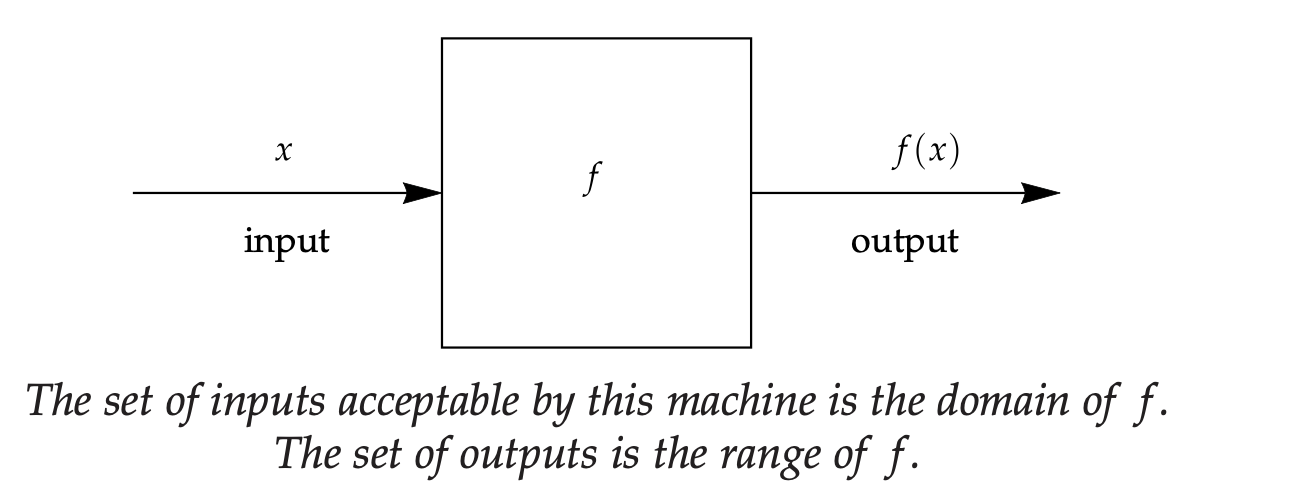
\includegraphics[scale=0.5]{function-engine.png}
\end{figure}
\end{frame}
\begin{frame}{Functions}
  \begin{exampleblock}{Example 4}
The domain of \(f\) is the interval \( [2, 5] \), with \(f\) defined on this interval by the equation \(f (x) = 3x + 1\)
  \end{exampleblock}
  Solution : \pause 
  \[
  y = f(x) = 3x+1 \]     \pause

  \[  2 \leq \frac{y-1}{3} \leq 5.  \pause
  \]

  \[  7 \leq y \leq 16.   \pause
   \]
\end{frame}
\begin{frame}{Function}
  \begin{exampleblock}{Example 5}
    The domain of \(g\) is the interval \([1,20]\), with \(g\) defined on this interval by
    the equation
    \[
    g(x) = |x - 5|.
    \]
    Is \(2\) in the range of \(g\)?
  \end{exampleblock}
  Solution :  \pause 
  \[ y =  |x-5| \]
  for \(x-5>0 \) ,\(y = x-5 \implies x = y+5 \)  
  \[ 5 < y+5 \leq 20  \implies  0 < y \leq 15 \]
  for \(x-5<0 \), \(y = -(x-5) \implies y = -x+5 \implies 5-y = x \)
  \[ 1 \leq 5-y \leq 5  \implies -4 \leq -y \leq 0 \implies  4 \geq y \geq 0 \] 
\end{frame}
\begin{frame}{Equality of Functions}
  \begin{beamercolorbox}[wd=\textwidth,rounded=true,shadow=true]{mycolorbox}
    Two functions are equal if and only if they have the same domain and the same value at every number in that domain
  \end{beamercolorbox}
  \begin{exampleblock}{Example}
    Suppose \(f\) is the function whose domain is the set of real numbers, with \(f\) defined
    on this domain by
    \[f (x) = x^2\]
    Suppose \(g\) is the function whose domain is the set of positive numbers, with \(g\)
    defined on this domain by
    \[g(x) = x^2\]
    Are \(f\) and \(g\) equal functions ?
  \end{exampleblock}
\end{frame}
\begin{frame}{Equality of functions}
  \begin{exampleblock}{Example 2}
    Suppose \(f\) and \(g\) are functions whose domain is the set consisting of the two numbers \(\{1, 2\}\) with \(f\) and \(g\) defined on this domain by the formulas
\[f (x) = x^2\] and \[g(x) = 3x-2\].Are \(f\) and \(g\) equal functions?
  \end{exampleblock}
\end{frame}
\subsection{Analytical Geometry}
\begin{frame}{What is Analytic Geometry?}
  \begin{itemize}
      \item \textbf{Analytic Geometry} (also called \textit{coordinate geometry} or \textit{Cartesian geometry}) bridges algebra and geometry.
      \item It uses a coordinate system to study geometric shapes and properties.
      \item Geometric objects are represented as algebraic equations.
  \end{itemize}
\end{frame}
\begin{frame}
  \frametitle{Co-ordinate Plane}
  \begin{figure}[h]    
      \centering
      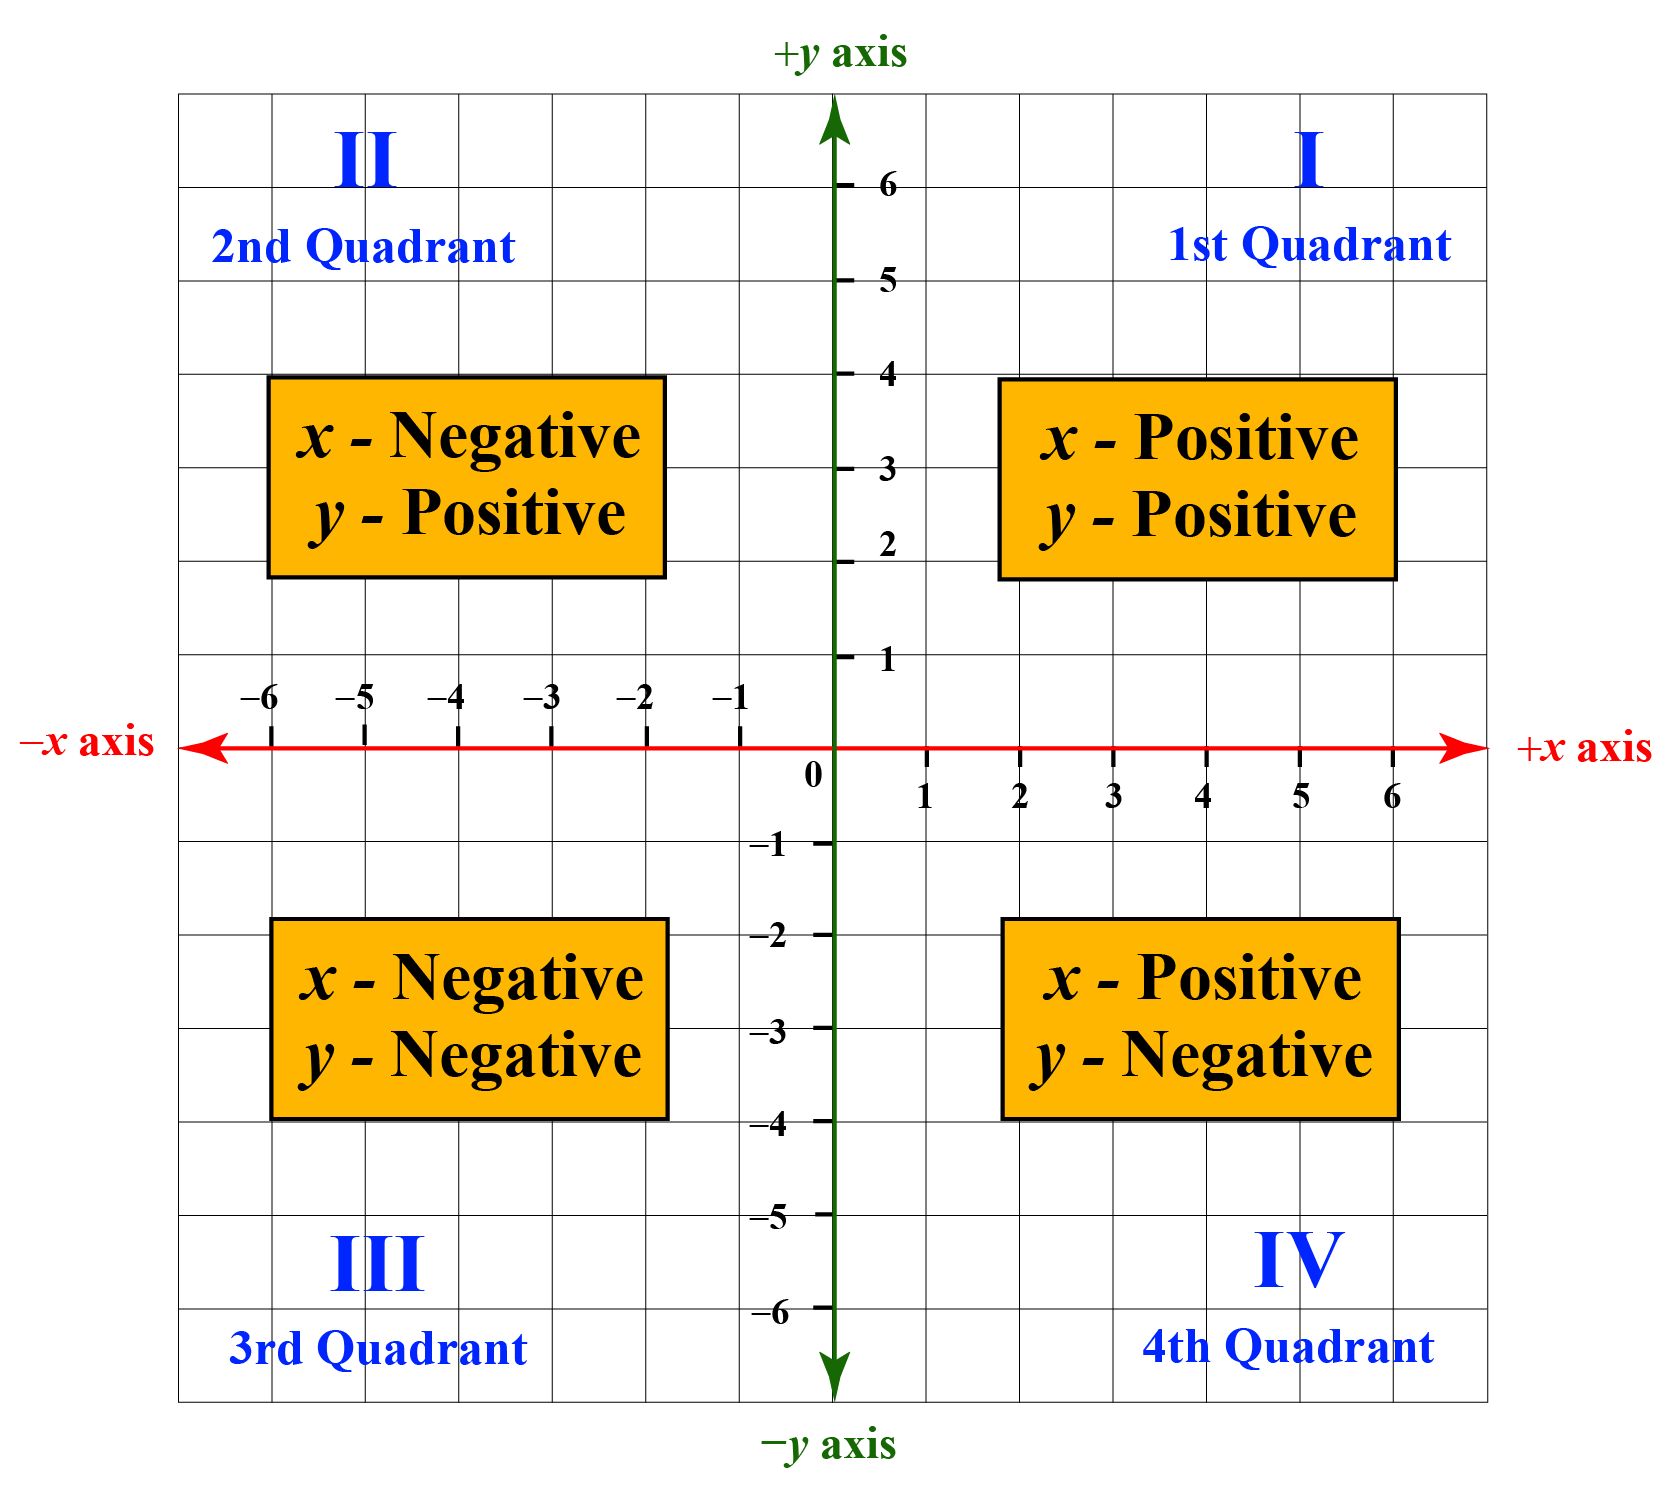
\includegraphics[scale=0.23]{cartesian.png}
\end{figure}
The plane with this system of labeling is often called the \textbf{Cartesian plane} in honor of the French mathematician Rene Descartes(1596-1650), who described this technique in his 1637 book Discourse on Method
\end{frame}
\begin{frame}{Graph Functions}
  \begin{beamercolorbox}[wd=\textwidth,rounded=true,shadow=true]{mycolorbox}
The graph of a function \(f\) is the set of points of the form \(x, f (x)\) as x varies
over the domain of \(f\)
  \end{beamercolorbox}
\end{frame}
\subsubsection{Graphs}
\begin{frame}
  \frametitle{Graph of a Function}
  \begin{figure}[h]    
    \centering
    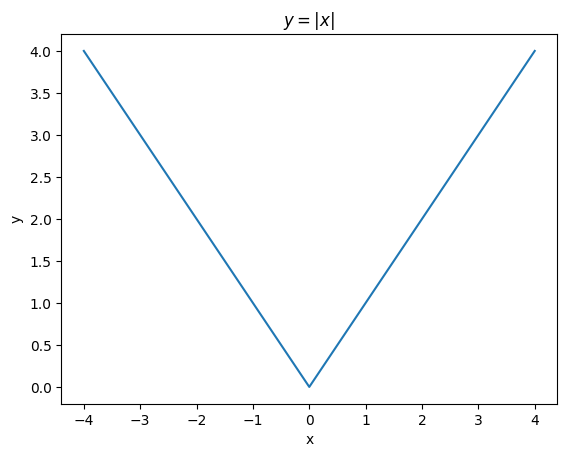
\includegraphics[scale=0.3]{graph.png}
\end{figure}
\begin{figure}[h]    
  \centering
  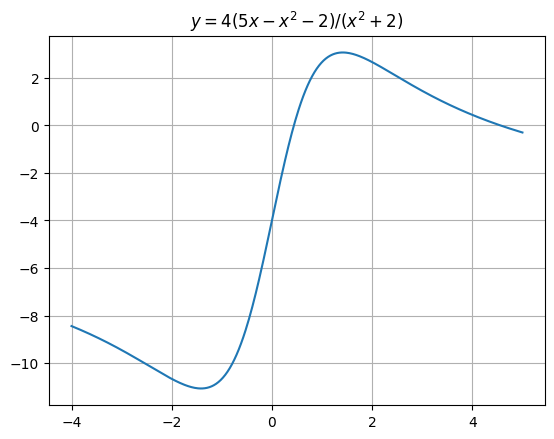
\includegraphics[scale=0.3]{graph2.png}
\end{figure}
\end{frame}

\begin{frame}
  \frametitle{Checking for a function: Vertical line test}
  \begin{figure}[h]    
  \centering
  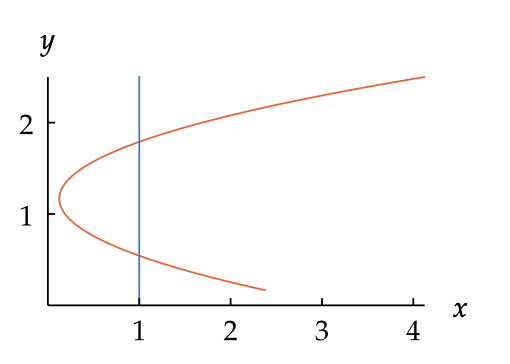
\includegraphics[scale=0.5]{not-fn.png}
  \end{figure}
  \pause
  The line  \(x=1\) intersects the curve at two points. That is that for each \(x\) value there are multiple \(y\) values which is contradicting to definition of a function 
  \begin{block}{Vertical Line Test}
    A set of points in the coordinate plane is the graph of some function if and only if every vertical line intersects the set in at most one point 
  \end{block}
\end{frame} 
\subsection{Function Transformation}
\begin{frame}
  \frametitle{Vertical Transformations}

  \begin{block}{Shifting a graph up or down}
    Suppose \(f \) is a function and \(a > 0\). Upshift \(g\) and  Downshift \(h\) by
\[g(x) = f (x) + a \;\; h(x) = f (x) - a \]
  \end{block}
  \frametitle{Vertical Transformation}
  \begin{figure}[h]    
    \centering
    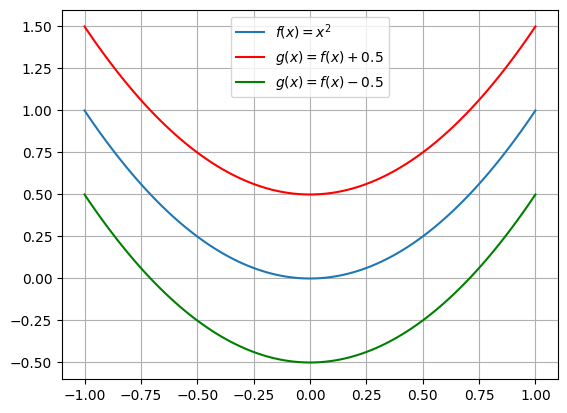
\includegraphics[scale=0.4]{vertical_shift.png}
    \end{figure}
\end{frame}
\begin{frame}
  \frametitle{Vertical Transformation}
  \begin{block}{Vertical Stretch}
    Suppose \(f\) is a function and \(c > 0\). Define a function \(g\) by
\[g(x) = c f (x)\]
  \end{block}
  \begin{figure}[h]    
    \centering
    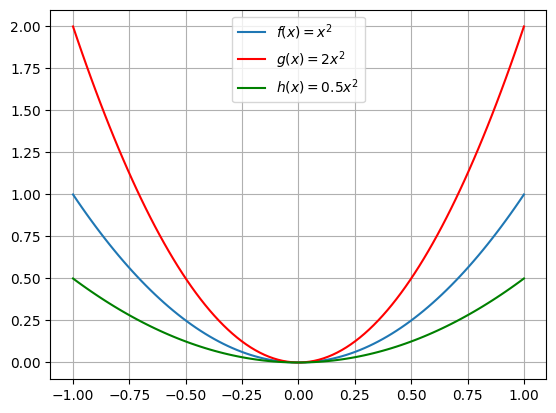
\includegraphics[scale=0.5]{vertical_stretch.png}
    \end{figure}
\end{frame}
\begin{frame}
  \frametitle{Vertical Transformation}
  \begin{block}{Flipping along the Vertical Axis} 
    Vertical fliiping of \(f(x) \) is 
    \[g(x) = - f (x) \]
  \end{block}
  \begin{figure}[h]    
    \centering
    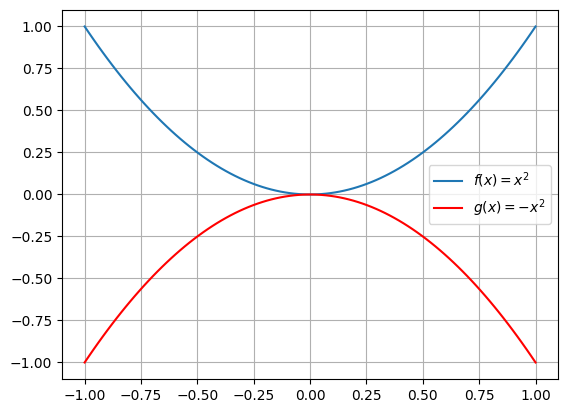
\includegraphics[scale=0.5]{vertical_flip.png}
    \end{figure}
\end{frame}
\begin{frame}
  \frametitle{Horizontal Transformation}
  \begin{block}{Horizontal Shift}
    \[g(x) = f(x+a), h(x) = f(x-a)\]
  \end{block}
  \begin{figure}[h]    
    \centering
    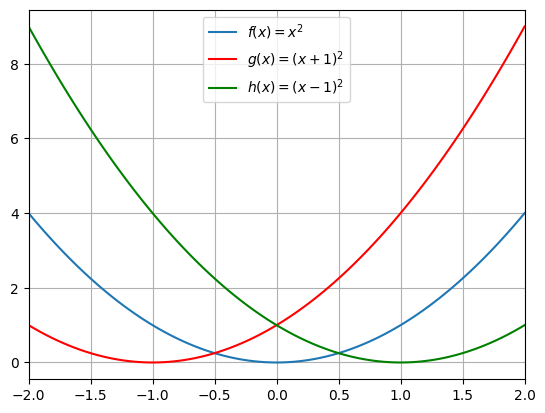
\includegraphics[scale=0.5]{horizontal-shift.png}
    \end{figure}
  \end{frame}
\begin{frame}
    \frametitle{Horizontal Transformation}
    \begin{block}{Horizontal Stretching}
      \[g(x) = f(cx)\]
    \end{block}
    \begin{figure}[h]    
      \centering
      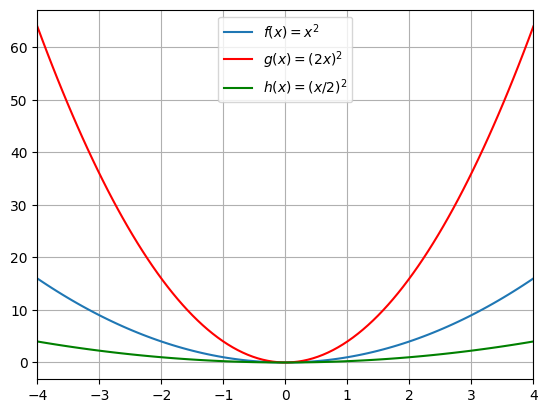
\includegraphics[scale=0.55]{horizontal-stretch.png}
      \end{figure}
\end{frame}
\begin{frame}
  \frametitle{Flipping ac the Vertical Axis}
  \begin{block}{Horizontal Stretching}
    \[g(x) = f(-x)\]
  \end{block}
  \begin{figure}[h]    
    \centering
    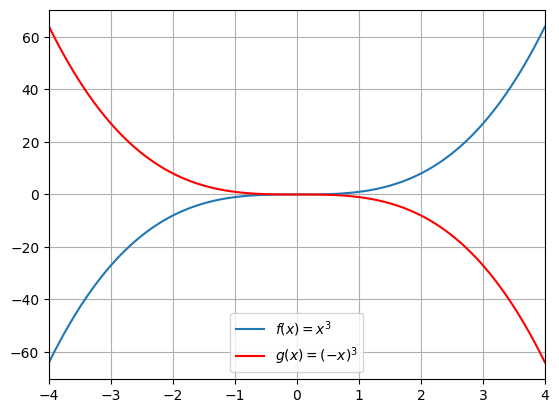
\includegraphics[scale=0.55]{vertical-axis-flip.png}
    \end{figure}
\end{frame}
\begin{frame}
  \frametitle{Combinations of vertical Transformation}
  \begin{figure}[h]    
    \centering
    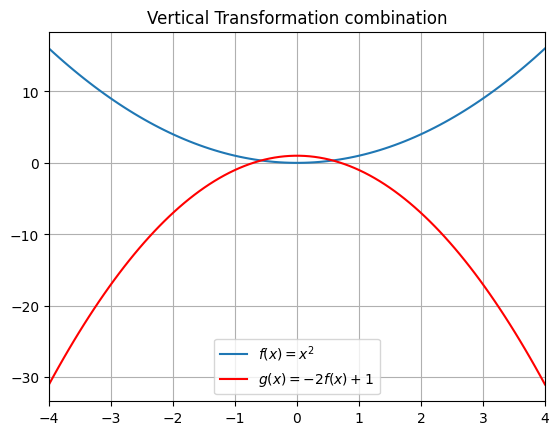
\includegraphics[scale=0.55]{vertical_combination.png}
    \end{figure}
\end{frame}
\begin{frame}{Even Functions}  
\begin{block}{Even}
        \[
        f(-x) = f(x) \quad \text{for all } x \text{ in the domain}
        \]
        Example: \( f(x) = x^2, \quad f(x) = \cos x \)
\end{block}
The graph of an even function is symmetric across the vertical axis 
\end{frame}
\begin{frame}
  \frametitle{Even Functions}
  \begin{columns}
    \column{0.5\textwidth}
    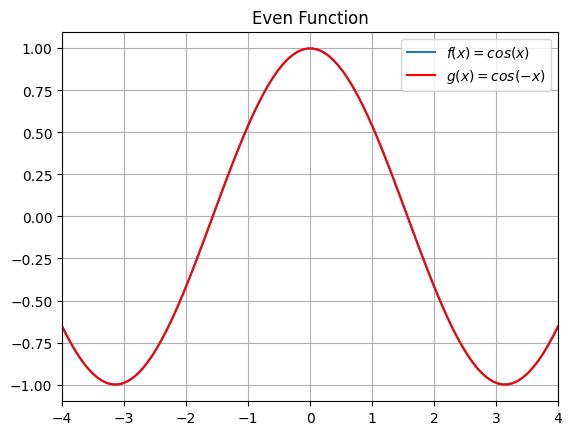
\includegraphics[width=\linewidth]{even.png}

    \column{0.5\textwidth}
    \centering
    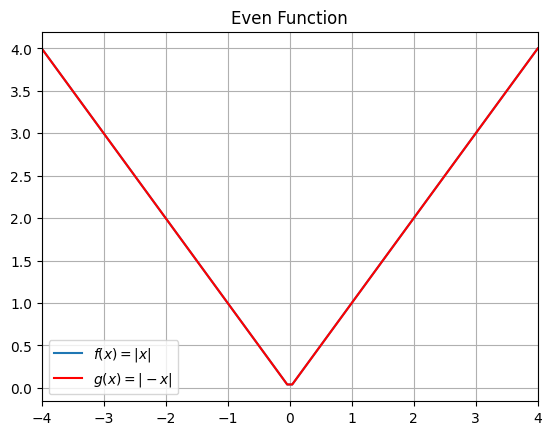
\includegraphics[width=\linewidth]{even2.png}
\end{columns}
\end{frame}
\begin{frame}{Odd Function}
\begin{block}{Odd}
        \[
        f(-x) = -f(x) \quad \text{for all } x \text{ in the domain}
        \]
        Example: \( f(x) = x^3, \quad f(x) = \sin x \)
\end{block}
The graph of an even function is symmetric if flipped or rotated 18 across the origin 
\end{frame}

\begin{frame}
  \frametitle{Odd Function}
  \begin{columns}[T]
    \begin{column}{0.5\textwidth}
    \begin{figure}[t]
    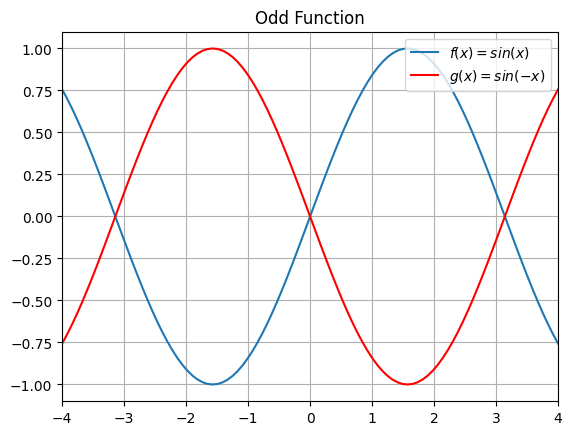
\includegraphics[width=\linewidth]{odd.png}
    \end{figure}
  \end{column}

  \begin{column}{0.5\textwidth}
    \begin{figure}[t]
    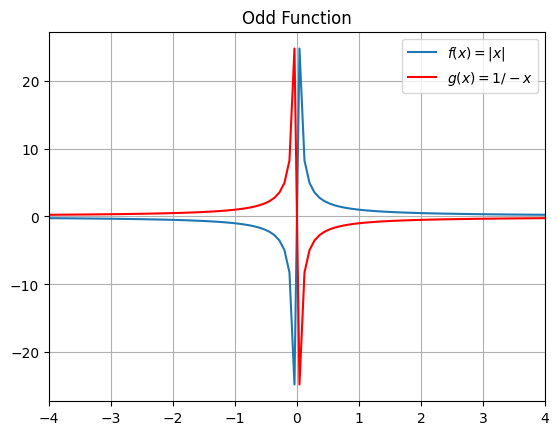
\includegraphics[width=\linewidth]{odd2.png}
    \end{figure}
  \end{column}
\end{columns}
\end{frame}

\subsection{Function Composition}
\begin{frame}
  \frametitle{Algebra of Functions} 
    Suppose \(f\) and \(g\) are functions. We can define new functions from \(f\) and \(g\) as follows: \\
  
  \pause
    \textbf{Sum:}  
    \[
    (f+g)(x) = f(x) + g(x)
    \]
    
    \pause
    \textbf{Difference:}  
    \[
    (f-g)(x) = f(x) - g(x)
    \]
    
    \pause
    \textbf{Product:}  
    \[
    (f\cdot g)(x) = f(x) \cdot g(x)
    \]
    
    \pause
    \textbf{Quotient:}  
    \[
    \left(\frac{f}{g}\right)(x) = \frac{f(x)}{g(x)} \quad \text{provided } g(x) \neq 0.
    \]
    \textbf{Note:} If \(f\) and \(g\) have domains \(D_f\) and \(D_g\), then these operations are defined on the intersection \(D_f \cap D_g\). In the case of the quotient, it is defined on
    \[
    \{x \in D_f \cap D_g : g(x) \neq 0\}.
    \]
    
  \end{frame}

  \begin{frame}
    \frametitle{Exercise }
    \( f(x)  = \sqrt{x-3}\) and \(g(x) = \sqrt{8 - x }\)
    
    Evaluate
    \begin{enumerate}
      \item[a.] \((f+g)(x)\)  
      \item[b.]  \((fg)(x)\)
      \item[c.] Find the domain of above 
    \end{enumerate}
  \pause 
  Sol: 
  \begin{enumerate}
    \item[a.] \(\sqrt{x-3} + \sqrt{8-x} \) 
    \item[b.] \(\sqrt{(x-3)(8-x)} \)  
    \item[c.]  Domian of \begin{enumerate}
      \item[a.] \(x\geq 3 \)  
      \item[b.] \(x \leq 8 \)  
      \item[c.] \( 3 \leq x \leq 8 \)    
    \end{enumerate}
  \end{enumerate}
\end{frame}
  \begin{frame}{Function Composition }
    \begin{block}{Definition:}  
    If \( f(x) \) and \( g(x) \) are functions, then the composition of \( f \) and \( g \), denoted by \( f \circ g \), is defined by
    \[
      (f \circ g)(x) = f(g(x)).
    \]
    \end{block}
    \medskip
    
    \textbf{Example:}
    Consider the function
    \[
      h(x) = \sqrt{x+3}.
    \]
    We can express \( h(x) \) as a composition of two functions \( f \) and \( g \) where:
    \[
      f(x) = \sqrt{x} \quad \text{and} \quad g(x) = x+3.
    \]
    
    Then,
    \[
      h(x) = f(g(x)) = f(x+3) = \sqrt{x+3}.
    \]
  \end{frame}
\begin{frame}
  \frametitle{Exercise}
  \(
  f(x) = \frac{1}{x-4} 
  \) and \( g(x) = x^{2} \) 
  \begin{enumerate}
    \item \(f \circ g \)  
    \item \( g \circ f \)   
    \item domian of \(f \circ g \) 
    \item domain of \( g \circ f \) 
  \end{enumerate}
  Sol: \pause 
  \begin{enumerate}
    \item  \(f(g(x)) = \frac{1}{x^{2} - 4}\)
    \item \(g(f(x)) = (\frac{1}{x-4})^{2}\) 
    \item \(R - \{-2,2\} \)  
    \item \(R - \{4\} \)  
  \end{enumerate}
\end{frame}
\begin{frame}
  \frametitle{Composition Machine}
\begin{figure}
  \centering 
  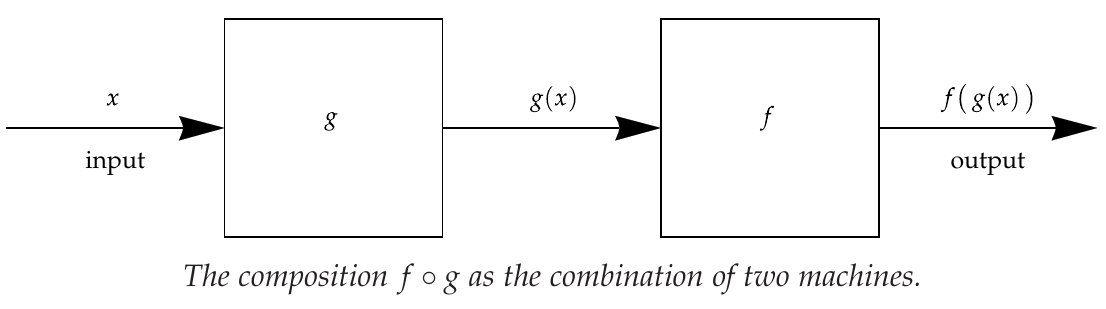
\includegraphics[scale=0.3]{composition.png}
\end{figure}
\end{frame}
\begin{frame}{Excersise}
  \textbf{Problem:} Suppose your cell phone company charges \$0.05 per minute plus \$0.47 for each call to China.
  \begin{enumerate}
    \item[(a)] Find a function \(p\) that gives the amount charged by your cell phone company for a call to China as a function of the number of minutes \(m\).
    \item[(b)] Suppose the tax on cell phone bills is 6\% plus \$0.01 for each call. Find a function \(t\) that gives your total cost, including tax, for a call to China as a function of the amount charged by your cell phone company.
    \item[(c)] Explain why the composition \(t \circ p\) gives your total cost, including tax, of making a cell phone call to China as a function of the number of minutes.
    \item[(d)] Compute a formula for \(t \circ p\).
    \item[(e)] What is your total cost for a ten-minute call to China?
  \end{enumerate}
  \end{frame} 
  \begin{frame}
    \frametitle{Solution}
    
    \textbf{(a)} The company charges \$0.05 per minute plus a fixed charge of \$0.47 per call. Hence, the pre-tax charge function is
    \[
    p(m)=0.05m+0.47.
    \]
    
    \textbf{(b)} The tax on the cell phone bill is 6\% of the pre-tax amount plus an additional \$0.01 per call. Thus, if the pre-tax charge is \(x\), the total cost function (including tax) is
    \[
    t(x)=1.06x+0.01.
    \]
    
    \textbf{(c)} The composition \(t \circ p\) means we first compute the pre-tax charge \(p(m)\) for a call of \(m\) minutes, and then we apply the tax function \(t\) to this amount. In other words, \(t(p(m))\) gives the total cost, including tax, as a function of the number of minutes.
    
    
    \textbf{(d)} To compute the composition, substitute \(p(m)\) into \(t\):
    \[
    (t \circ p)(m)=t(p(m))=1.06\bigl(0.05m+0.47\bigr)+0.01.
    \]
  \end{frame}
  \begin{frame}
    \frametitle{Solution}
    Distribute \(1.06\):
    \[
    1.06(0.05m)=0.053m \quad \text{and} \quad 1.06(0.47)=0.4982.
    \]
    Thus,
    \[
    (t \circ p)(m)=0.053m+0.4982+0.01=0.053m+0.5082.
    \]
    \textbf{(e)} For a ten-minute call (\(m=10\)):
    \[
    (t \circ p)(10)=0.053(10)+0.5082=0.53+0.5082=1.0382.
    \]
    Rounded to the nearest cent, the total cost is approximately \$1.04.
  \end{frame}
  \begin{frame}
    \frametitle{}
    \begin{block}{Identity Function}
      The identity function is defined by
      \[
      I(x) = x \quad \text{for every number } x.
      \]
      \end{block}

      \begin{alertblock}{The function \(I\) is the identity for composition}
        If \(f\) is any function, then
        \[
        f \circ I = I \circ f = f.
        \]
        \end{alertblock}
  \end{frame}
\begin{frame}
  \frametitle{Decomposing the Functions}
  \begin{exampleblock}{Function Decomposition}
    \[
    T(y) = \frac{|y^{2} -3|}{|y^{2} - 7|}
    \]
    Sol: \pause
    \medskip 
    \[f(y) = |y|, g(y) = \frac{y^{2}-3}{y^{2}-7} \]
    \[ f(y) = \frac{|y-3|}{|y-7|}, g(y) = y^{2}\]
  \end{exampleblock}
  \begin{alertblock}{Composition is associative}
    if \(f,g, h\) are functions then 
    \[(f \circ g) \circ h  = f \circ (g \circ h) \]
  \end{alertblock}
\end{frame}
\begin{frame}
  \frametitle{Example}
  \begin{exampleblock}{Composition of three functions}

    \[T(x) = \left| \frac{x^{2}-3}{x^{2} - 7}  \right| \]

    Sol: \pause
     \[f(x) = |x|, g(x) = \frac{x-3}{x-7}, h(x) = x^{2}\]
    
  \end{exampleblock}
\end{frame}
\begin{frame}
  \frametitle{Linear Functions}
  \begin{block}{Linear Function}
    A linear function is a function \(h\) of the form 
    \[h(x) = mx + b\]
    where \(m\) and \(b\) are numbers
  \end{block}
\end{frame}

\begin{frame}
  \frametitle{Linear Functions as Composition}
  \begin{exampleblock}{Vertical Transformations as Compositions}
    A funtion \(g(x)\) is defined by 
    \[g(x)= -2f(x)+1\] 
    Write \(g(x)\) as a the composition of a linear function with \(f(x)\) 
    \[h(x) = -2x + 1 \]
    \[\implies g(x) = h(f(x)) \implies g = h \circ f \]
   \end{exampleblock}
  \end{frame}
  \begin{frame}{Linear Function as Composition}
   \begin{exampleblock}{Horizontal Transformations as Compositions}
    A funtion \(g(x)\) is defined by 
    \[g(x)= f(2x)+1\] 
    Write \(g(x)\) as a the composition of a linear function,  \(f(x)\) and other linear function 
    \[h(x) = x + 1, p(x) = 2x \]
    \[\implies g(x) = h(f(p(x))) \implies g = h \circ f \circ p \]
   \end{exampleblock}
\end{frame}
\subsection{Inverse Functions}
  \begin{frame}
    \frametitle{Inverse Function: Example}
      Consider the function \( f: \mathbb{R} \to \mathbb{R} \) defined by
      \[
      y = \frac{9}{5}x + 32,
      \]
      which converts a temperature \( x \) in Celsius to Fahrenheit \( y \).
      The inverse function \( f^{-1} \) converts Fahrenheit back to Celsius:
      \[
      f^{-1}(y) = \frac{5}{9}(y - 32).
      \]
      Verifying that these functions are inverses:
      \[
      f^{-1}(f(x)) = \frac{5}{9}\Bigl(\frac{9}{5}x + 32 - 32\Bigr) = x,
      \]
      \[
      f(f^{-1}(f)) = \frac{9}{5}\Bigl(\frac{5}{9}(y - 32)\Bigr) + 32 = y.
      \]
  \end{frame}
\begin{frame}
  \frametitle{One-to-One Function}
  \begin{block}{One-to-One Function}
    A function \(f\) is called one-to-one if for each number \(y\) in the range of \(f\) there is
  exactly one number \(x\) in the domain of \(f\) such that \(f (x) = y\)
  \end{block}
\end{frame}

\begin{frame}
  \frametitle{Inverse Function}
  \begin{block}{Definition}
    Suppose \( f \) is a one-to-one function.
    \begin{itemize}
      \item If \( y \) is in the range of \( f \), then \( f^{-1}(y) \) is defined to be the number \( x \) such that \( f(x) = y \).
      \item The function \( f^{-1} \) is called the \emph{inverse function} of \( f \).
    \end{itemize}
    \vspace{1em}
    \textbf{Short version:}
    \begin{itemize}
      \item \( f^{-1}(y) = x \) means \( f(x) = y \).
    \end{itemize}
    \end{block}
\end{frame}
\begin{frame}
  \frametitle{Inverse Function}
\begin{figure}
  \centering
  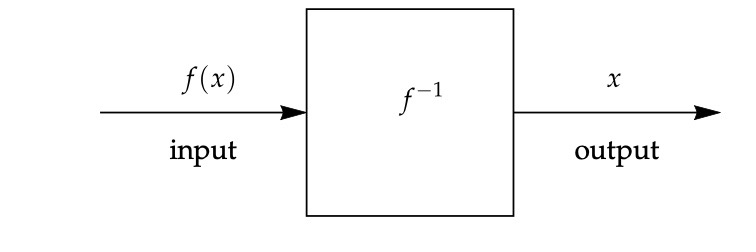
\includegraphics[scale=0.4]{inverse.jpeg}
\end{figure}
\end{frame}
\begin{frame}{Domain and Range of an Inverse Function}
  \begin{block}{Properties}
  If \( f \) is a one-to-one function, then:
  \begin{itemize}
    \item The domain of \( f^{-1} \) equals the range of \( f \).
    \item The range of \( f^{-1} \) equals the domain of \( f \).
  \end{itemize}
  \end{block}
  \end{frame}
  \begin{frame}
    \frametitle{Increasing and Decreasing Function}
    \begin{block}{Increasing}
      A function \(f\) is called increasing if \(f (a) < f (b)\) whenever \(a < b\) and \(a, b \) are in
the domain of \(f\)
    \end{block}
    \begin{block}{Decreasing}
      A function \(f\) is called decreasing if \(f (a) >  f (b)\) whenever \(a < b\) and \(a, b \) are in
the domain of \(f\)
    \end{block}
    \begin{alertblock}{Increasing and decreasing functions are one-to-one}
      \begin{itemize}
        \item Every increasing function is one-to-one
        \item Every decreasing function is one-to-one.
      \end{itemize}
    \end{alertblock}
  \end{frame}
  \begin{frame}
    \frametitle{Exercise}
    \begin{figure}
      \centering
      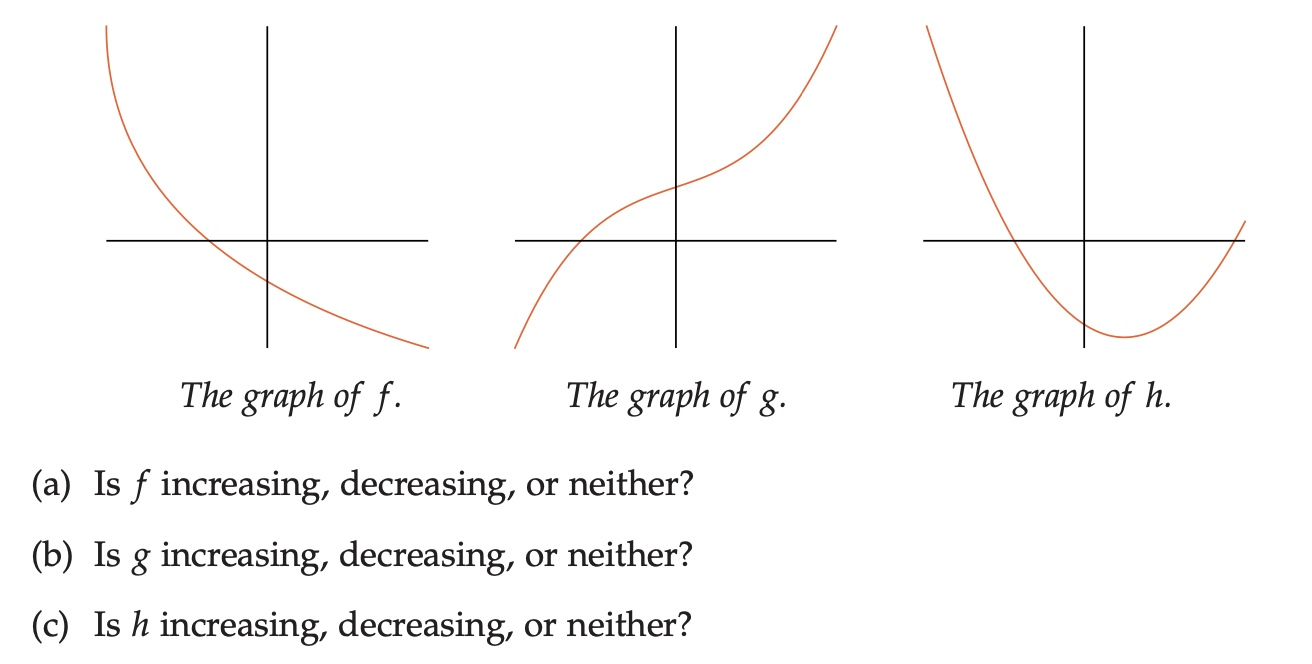
\includegraphics[scale=0.2]{increase.jpeg}
    \end{figure}
    \pause
  \begin{enumerate}
    \item[a.] Decreasing
    \item[b.] Increasing
    \item[c.] Neither
  \end{enumerate}
  \end{frame}
  \begin{frame}
    \frametitle{Do all one-to-one maps are increasing or decreasing ? }
    \begin{figure}
      \centering
      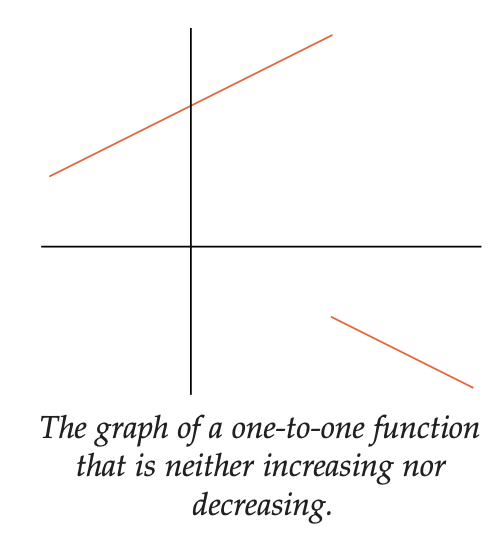
\includegraphics[scale=0.6]{non-increse-decrese.png}
    \end{figure}
  \end{frame}
  \begin{frame}{Increasing and Decreasing Functions}

    \begin{alertblock}{Inverses of increasing and decreasing functions}
      \begin{itemize}
        \item The inverse of an increasing function is increasing.
        \item The inverse of a decreasing function is decreasing.
      \end{itemize}
    \end{alertblock}
  \end{frame}
  \section{Linear,Quadratic, Polynomial and Rational Functions}
  \subsection{Lines and Linear Function}
  \begin{frame}{Slope}
    \begin{figure}
      \centering
      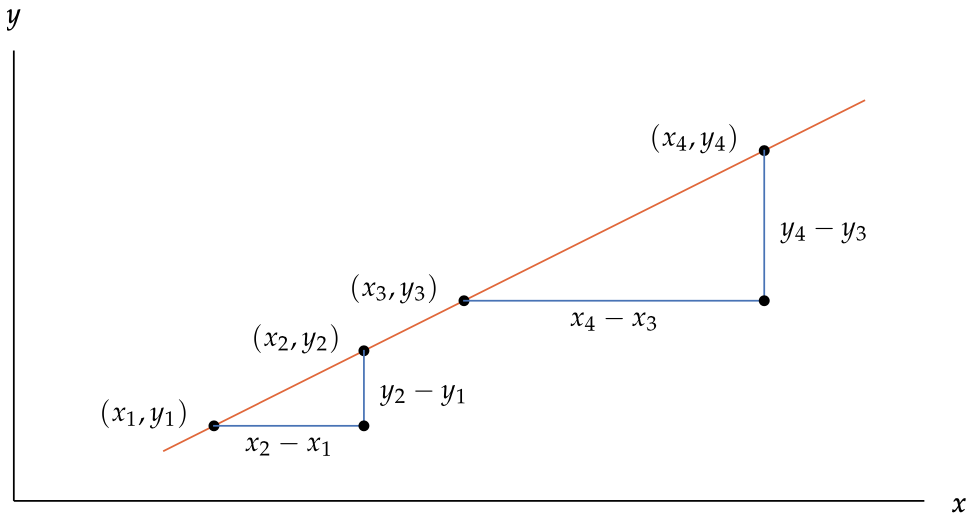
\includegraphics[scale=0.25]{slope.png}
    \end{figure}

    \[\frac{y_{2} - y_{1}}{x_{2} - x_{1}} = \frac{y_{4} - y_{3}}{x_{4} - x_{3}}\]
  \end{frame}
  \begin{frame}
    \frametitle{Slope}
    \begin{block}{Definition}
      If \(x_{1},y_{1}\) and \(x_{2},y_{2}\) are any two points on a line with \(x_{1} \neq x_{2}\), then the \textbf{slope}
      of the line is 
      \[\frac{y_{2} - y_{1}}{x_{2} - x_{1}}\] 
    \end{block}
  \end{frame}

  \begin{frame}
    \frametitle{Slope}
    
    \begin{columns} 
      \column{0.5\textwidth} 
      \textbf{Key Points:}
      \begin{itemize}
          \item Positive slope slands up from left to right 
          \item Negative slope slands down from left to right 
          \item Horizontal line has slope = 0
          \item Vertical line has no slope
      \end{itemize}
  
      \column{0.5\textwidth} % Right column - 50% width
      \centering
      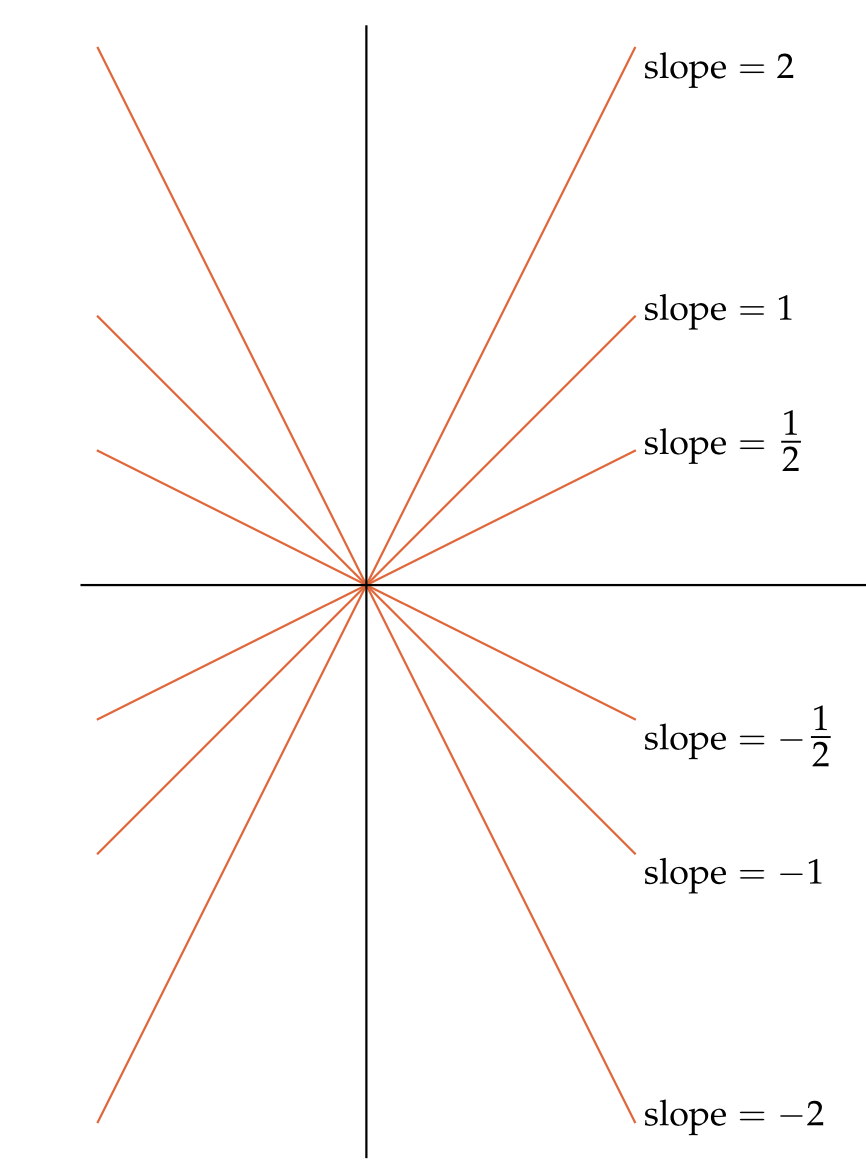
\includegraphics[width=0.8\linewidth]{slope2.png} % Replace with your image filename
  \end{columns}
  \end{frame}

\begin{frame}
  \frametitle{Line Equation}
  \begin{columns} 
    \column{0.5\textwidth} 
  \begin{alertblock}{slope and one point on it}
    The line in the xy-plane that has slope \(m\) and contains the point \((x1, y1)\) is given
by the equation 
\[y - y_{1} = m(x  -  x_{1})\]
  \end{alertblock}

  \column{0.5\textwidth} % Right column - 50% width
  \centering
  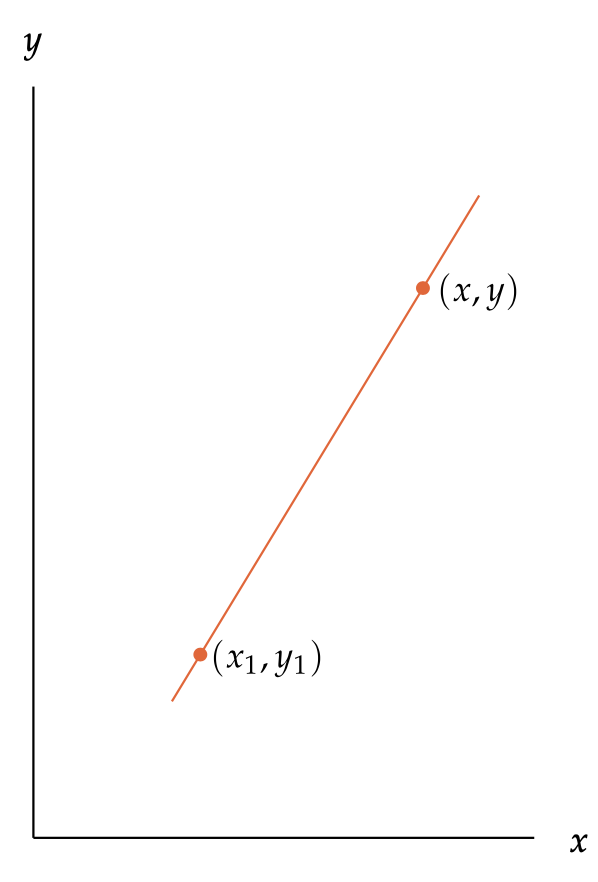
\includegraphics[width=0.8\linewidth]{line1.png} % Replace with your image filename
  \end{columns}

\end{frame}

\begin{frame}
  \frametitle{Line Equation}
  \begin{columns} 
    \column{0.5\textwidth} 
  \begin{alertblock}{slope and \(y\) intercept}
    The line in the xy-plane with slope \(m\) that intersects the \(y\) axis at \(0,b\) is given by the equation 
by the equation 
\[y = mx+b\]
  \end{alertblock}

  \column{0.5\textwidth} % Right column - 50% width
  \centering
  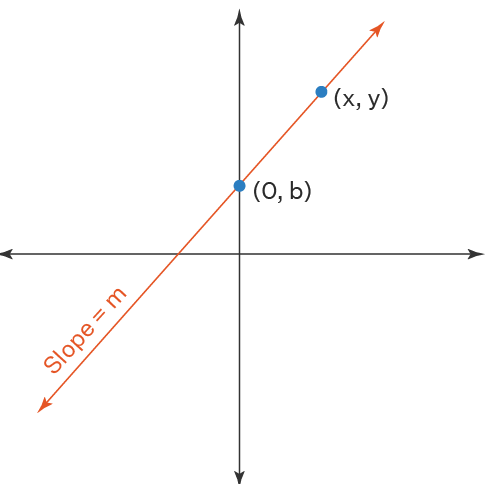
\includegraphics[width=0.8\linewidth]{line2.png} % Replace with your image filename
  \end{columns}

\end{frame}

\begin{frame}
  \frametitle{Line Equation}
  \begin{columns} 
    \column{0.5\textwidth} 
  \begin{alertblock}{slope and \(y\) intercept}
    The line in the xy-plane that contains the points \(x_{1},y_{1}\) and \(x_{2}, y_{2}\) where \(x_{1} \neq x_{2}\), is  
\[y = mx+b\], is given by the equation 
\[y-y_{1} = \left( \frac{y_{2} - y_{1}}{x_{2} - x_{1}} \right) (x-x_{1})\] 
  \end{alertblock}

  \column{0.5\textwidth} % Right column - 50% width
  \centering
  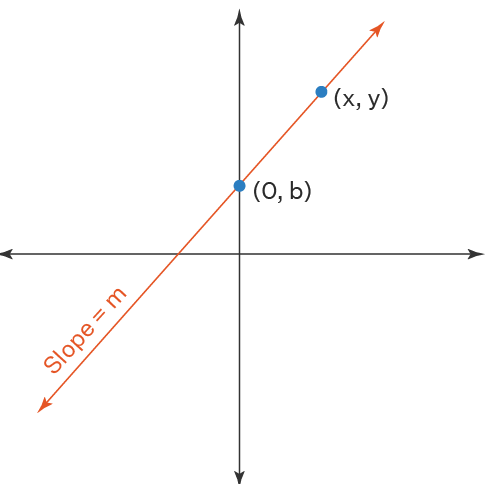
\includegraphics[width=0.8\linewidth]{line2.png} % Replace with your image filename
  \end{columns}

\end{frame}

\begin{frame}{Linear Function}
  \begin{block}{Definition}
    A \textbf{linear function} is a function \(f\) of the form 
    \[f(x) = mx + b\]
    where \(m\) and \(b\) are numbers
    
  \end{block}
\end{frame}

  \begin{frame}{Linear Functions: Origin vs Y-Intercept}

    \begin{columns}
        \column{0.5\textwidth} % Left Column - Text
        \textbf{Example 1: Temperature Conversion}
        \begin{itemize}
            \item Correct formula: \( F = 1.8C + 32 \) (Starts at 32°F)
            \item Incorrect direct proportion: \( F' = 1.8C \) (Wrong assumption)
        \end{itemize}
    
        \textbf{Example 2: Weight Conversion}
        \begin{itemize}
            \item True conversion: \( lb = 2.205 \times kg \) (Passes through origin)
            \item Shipping charge model: \( lb' = 5 + 2.205 \times kg \) (Has minimum billable weight or fixed cost markup)
        \end{itemize}
    
        \column{0.5\textwidth} % Right Column - Images
        \centering
        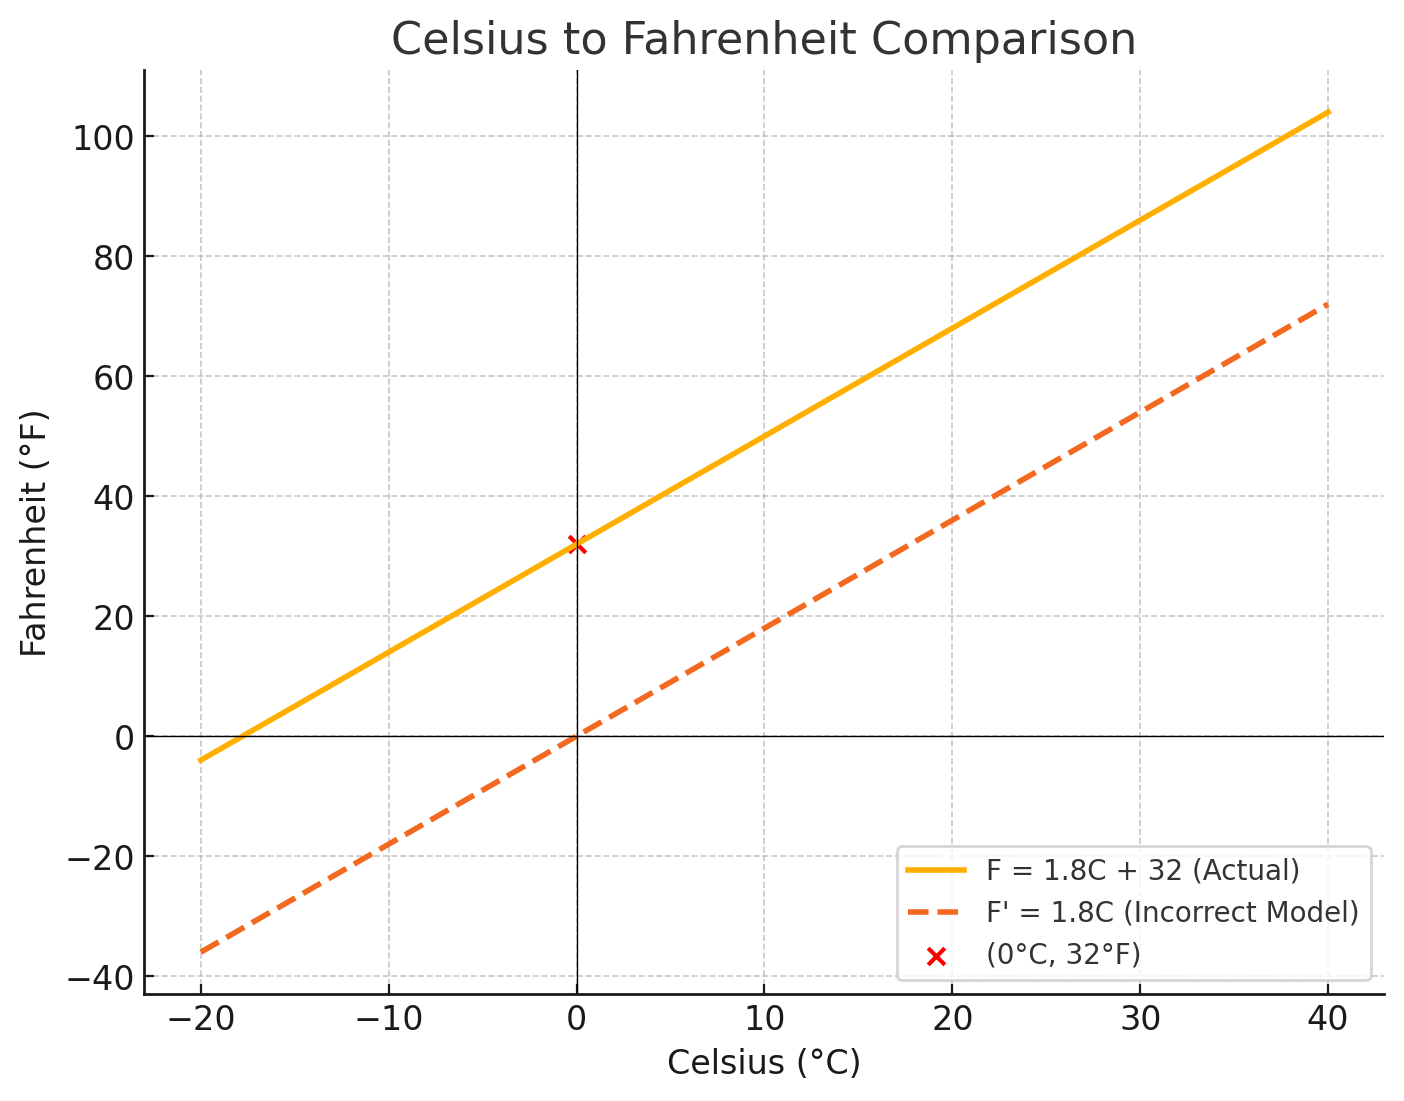
\includegraphics[width=0.8\linewidth]{Celsius to Fahrenheit Comparison.png} \\ % Replace with actual image
        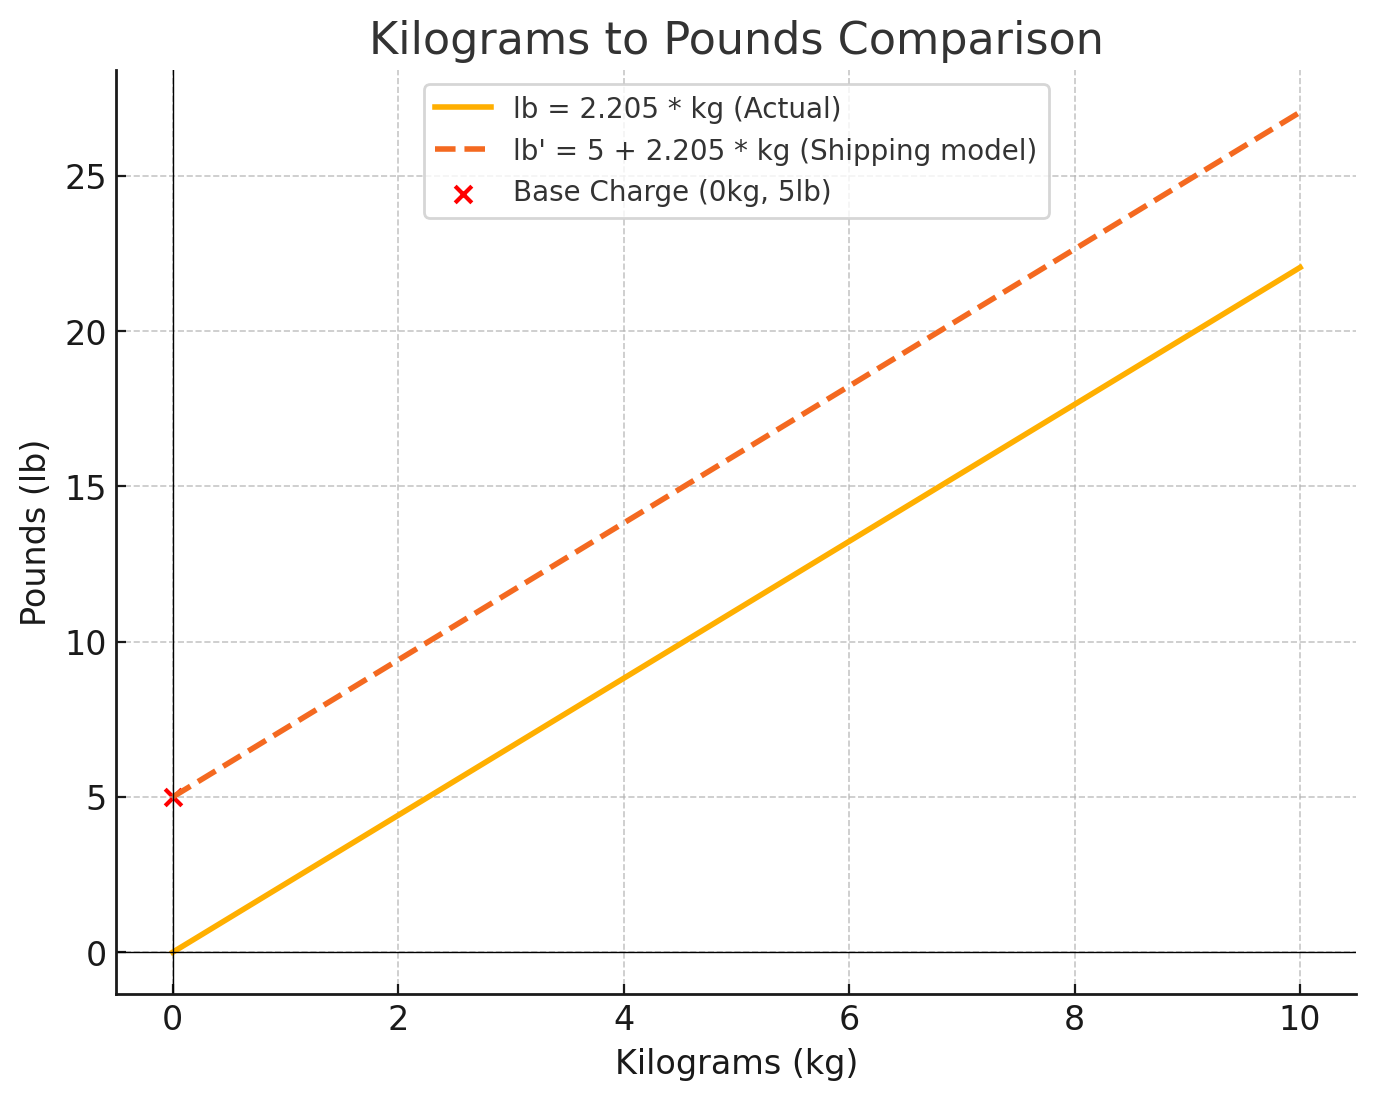
\includegraphics[width=0.8\linewidth]{Kilograms to Pounds Comparison.png} % Replace with actual image
    \end{columns}
    \end{frame}
\begin{frame}{Constant Function}
    \begin{block}{Definition}
      A constant function is a function \(f\) of the form \(f (x) = b\),  where \(b\) is a number 
    \end{block}
    \centering
    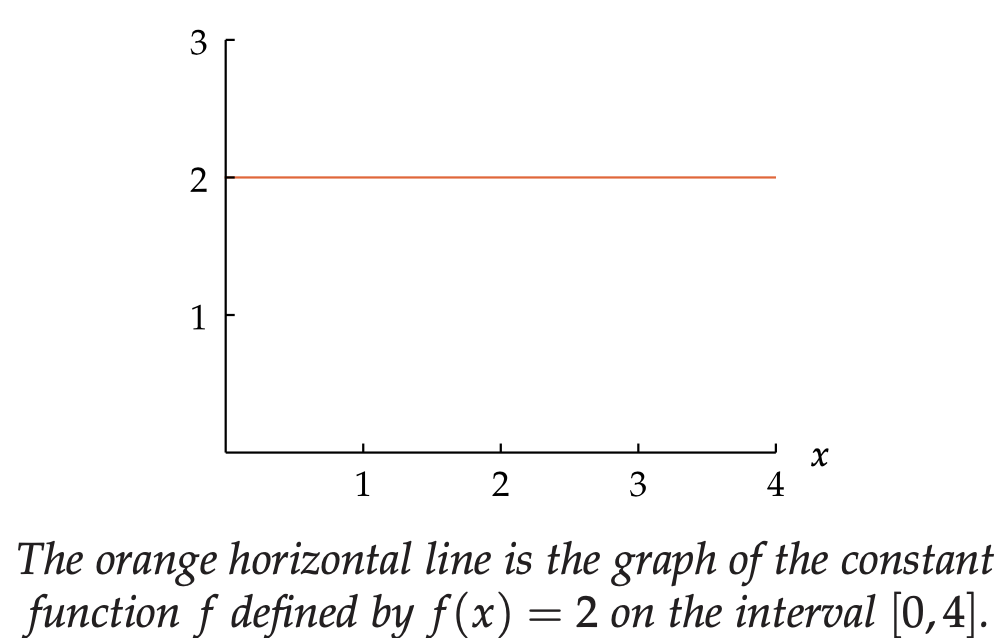
\includegraphics[width=0.6\linewidth]{constant.png} 
  \end{frame}

  \begin{frame}{Parallel Lines}
    \begin{figure}
      \centering
      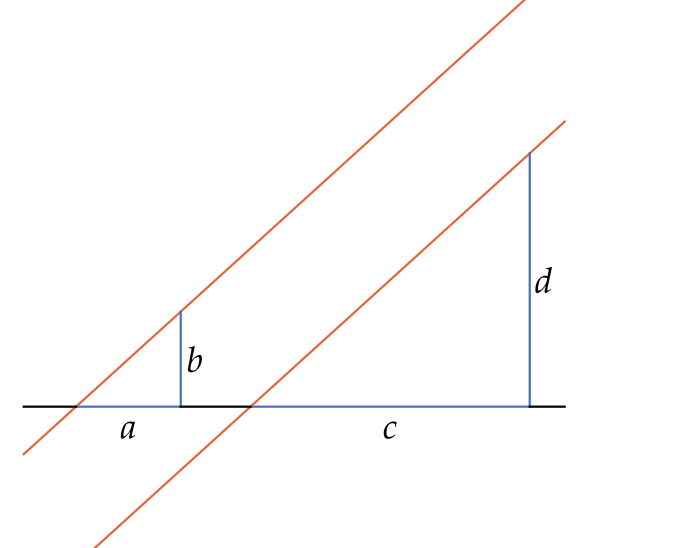
\includegraphics[scale=0.2]{parallel.png}
    \end{figure}
    As two lines are parallel, the corresponding angles are concurent and so two triangles are similar so 
\[\frac{a}{c} = \frac{b}{d} \implies \frac{b}{a} = \frac{d}{c}  \] 
it has same slope
  \end{frame}

  \begin{frame}{Negative Slope}
    \begin{figure}
      \centering
      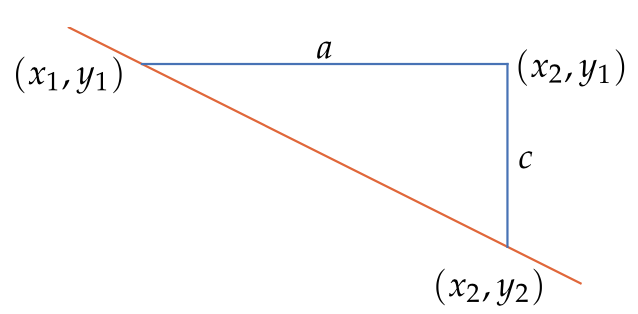
\includegraphics[scale=0.3]{negative-slope.png}
    \end{figure}
    As lengths are positive \(a = x_{2} - x_{1}\) and \(c = y_{1} - y_{2} \)  \\
    \bigskip
    Slope  = \(\frac{y_{2} - y_{1}}{x_{2} - x_{1}} = -\frac{c}{a} \) 
  \end{frame}

  \begin{frame}{Perpendicular Lines}
    \begin{columns}
      \column{0.5\textwidth} % Left Column - Text
      \(\triangle PSQ \) and \( \triangle TSP \) are similar \\ 

      \bigskip
      \(\frac{QS}{SP} = \frac{PS}{ST} \implies \frac{b}{a} = \frac{a}{c} \) \\

      \bigskip
      Multiplying by \(-\frac{c}{a} \implies \frac{b}{a} \cdot \left( - \frac{c}{a} \right) = -1  \) \\

      \column{0.5\textwidth} % Right Column - Images
      \centering
      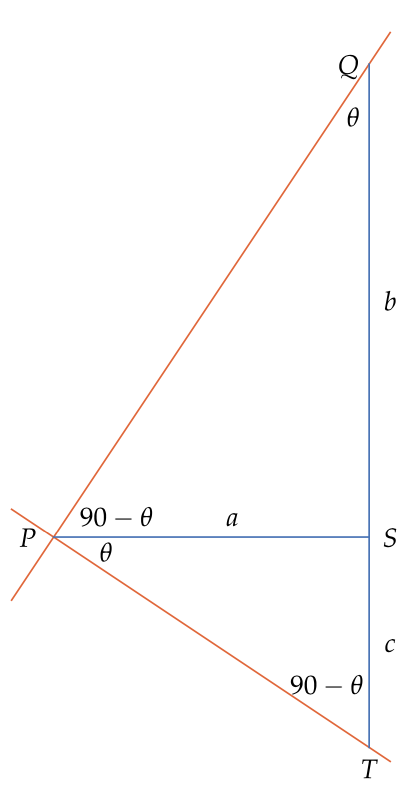
\includegraphics[width=0.5\linewidth]{perpendicular.png} \\ % Replace with actual image
  \end{columns}
  
  \end{frame} 

  \begin{frame}
    \frametitle{Unequal Scales}
    \begin{alertblock}{Angles are distorted by unequal scales on coordinate axes}
      In graphs with unequal scales on the two coordinate axes, angles are not
      accurately represented
    \end{alertblock}
    \begin{figure}
      \centering
      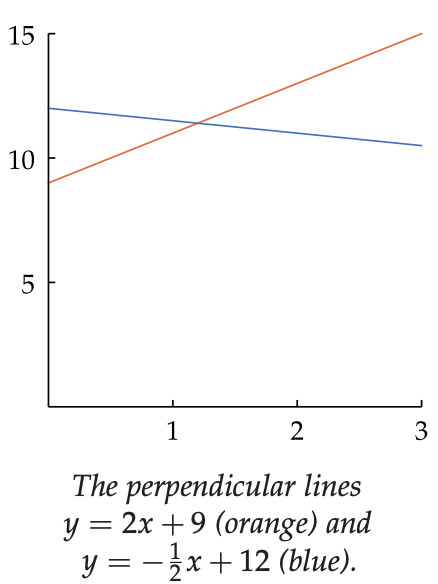
\includegraphics[scale=0.25]{unequal-scale.png}
    \end{figure}
  \end{frame}
  \subsection{Quadratic Functions and Conics}
  \begin{frame}{Conics}
    \begin{figure}
      \begin{center}
        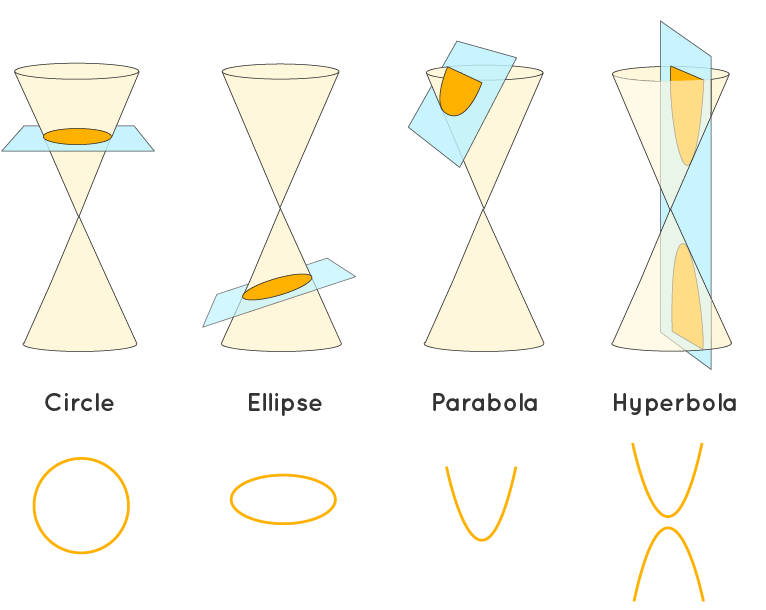
\includegraphics[scale = 0.3]{conic-section.png}
      \end{center}
    \end{figure}
  \end{frame}
  \begin{frame}
    \frametitle{Quadratic Function}
    \begin{block}{Definition}
      The function of the form 
      \[ax^{2} + bx + c = 0\]
      where \(a,b,c\) are real numbers with \(a \neq 0\)
      \begin{itemize}
        \item if \(b^{2} - 4ac < 0\), then equation have no real solutions
        \item if \(b^{2} - 4ac = 0\), then equation has one solution, \(x = -\frac{b}{2a}\)
        \item if \(b^{2} - 4ac  > 0\), then equation has two solutions \(x = \frac{-b \underset{-}{+}\sqrt{b^{2} - 4ac}}{2a}\)
      \end{itemize}
    \end{block}
  \end{frame}

  \begin{frame}
    \frametitle{Parabola}
    \begin{block}{Parabola}
      A \textbf{parabola} is the graph of a quadratic function. The \textbf{vertex} of the parabola is the where the line of symmetry of the parabola, intersects the parabola. \\ 

      \bigskip 
      Suppose \(f\) is a quadratic function. Complete the square to write \(f\) in the form 
      \[ f(x) = a(x-h)^{2} + k \] 
      \begin{itemize}
        \item If \(a > 0\) then \(f(x)\) attains its minimum value \(k\) when \(x=h\) and the graph of \(f\) is a parabola that opens upward.
        \item If \(a < 0 \) then \(f(x) \) its maximum value \(k\) when \(x=h\) and the graph of \(f\) is a parabola that opens downward 
        \item The vertex of the graph is \(h,k\)
      \end{itemize}

    \end{block}
  \end{frame}

  
  \begin{frame}
    \frametitle{Parabola}
   \begin{exampleblock}{Example}
    \[f(x) = -3x^{2} + 12x - 8 \]
    \begin{enumerate}
      \item For what value of \(x\) does \(f (x) \) attain its maximum value?
      \item What is the maximum value of \(f (x)\)?
      \item Find the vertex 
    \end{enumerate}
   \end{exampleblock}
   Sol: \\ 
   \[f(x) = -3x^{2} + 12x - 8 \implies -3(x^{2} - 4x + 4) + 4 \implies -3(x-2)^{2} + 4 \]
   \begin{enumerate}
    \item \(x = 2\)
    \item \(f(x=2) = 4\)
    \item \( (2,4) \)
   \end{enumerate}
  \end{frame}
 \begin{frame}
  \frametitle{Parabola}
  \begin{figure}
    \centering
    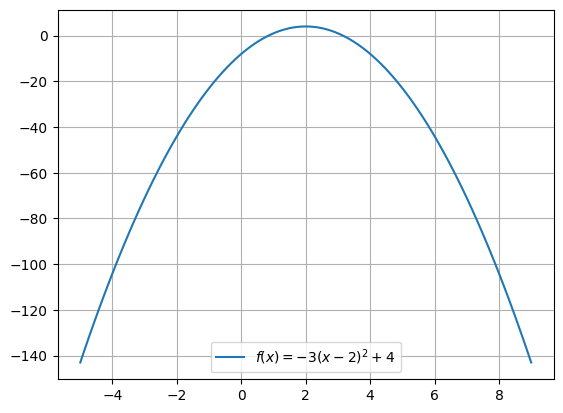
\includegraphics[scale=0.6]{parabola.png}
  \end{figure}
 \end{frame}

 \begin{frame}
  \frametitle{Distance Between Points}
  \begin{figure}
    \centering
    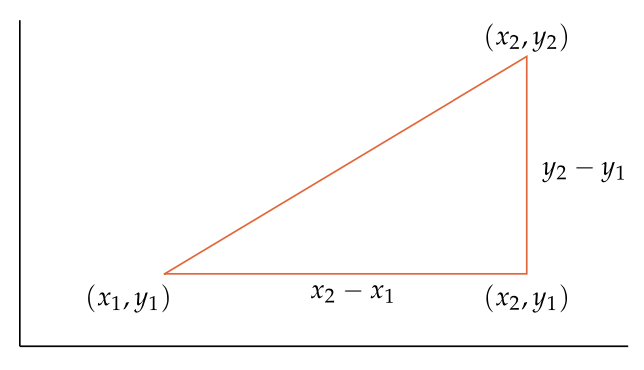
\includegraphics[scale=0.3]{distance-between-points.png}
  \end{figure}
 \begin{alertblock}{Distance Between Points}
  The distance between points \(x_{1}, y_{1}\) and \(x_{2}, y_{2}\) is given by 
  
  \[\sqrt{ \left(x_{2} - x_{1} \right)^{2}  + \left( y_{2} - y_{1} \right)^{2} }\]
  
 \end{alertblock}
 \end{frame}

 \begin{frame}
  \frametitle{Circle}
  \begin{block}{Equation of a Circle}
    The circle with center \(h,k\) and radius \(r\) is the set of the points \(x,y\) that satisfy the equation
    \[\left(x-h\right)^{2} + \left(y-k\right)^{2} = r^{2}\] 
  \end{block}
 \end{frame}

 \begin{frame}
  \frametitle{Ellispe}
  \begin{figure}
    \centering
    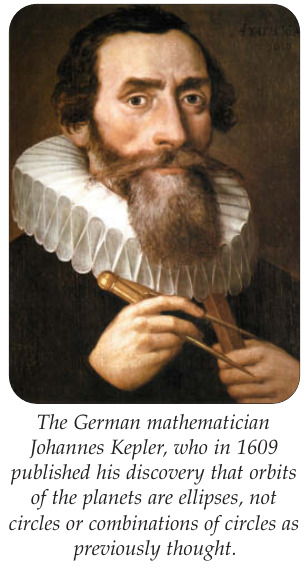
\includegraphics[scale=0.38]{ellipse0.png}
  \end{figure}
 \end{frame}


 \begin{frame}
  \frametitle{Ellipses}
  \begin{block}{Ellipse}
    Stretching the circle horizontally and/or vertically produces a curve called an \textbf{ellipse}
  \end{block}
  \begin{figure}
    \centering 
    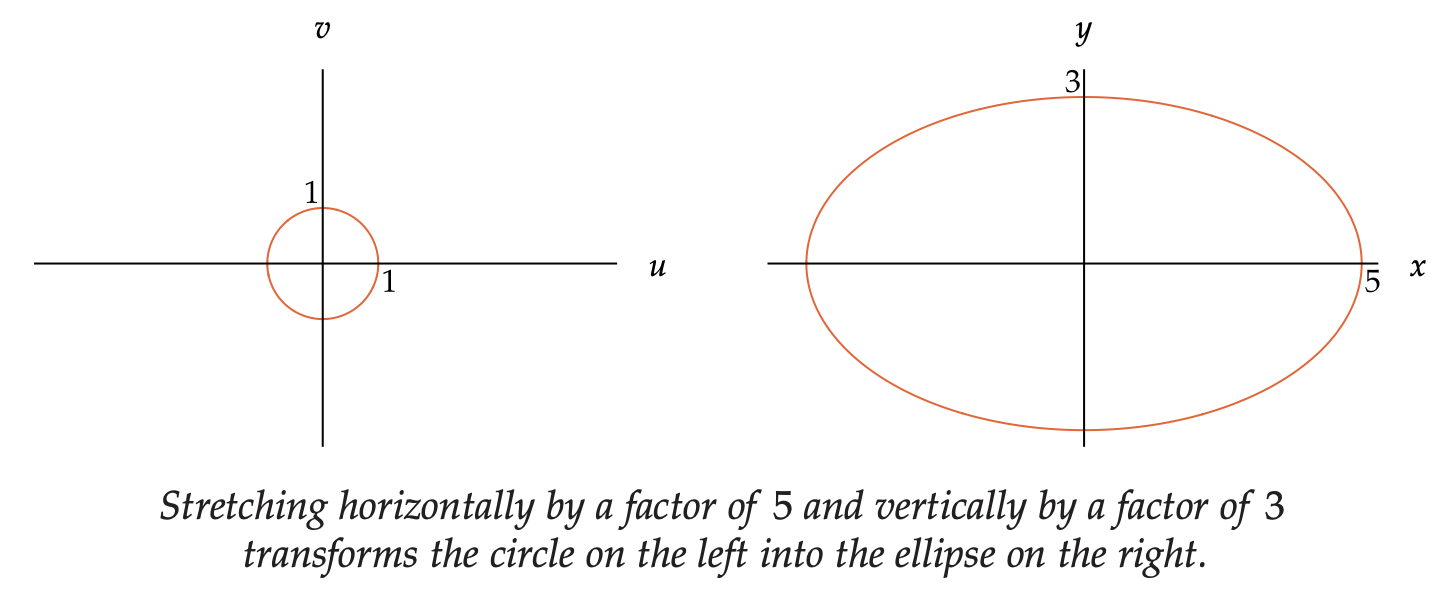
\includegraphics[scale=0.4]{ellipse.png}
  \end{figure}
 \end{frame}
 


 \begin{frame}
  \frametitle{Ellispe}
\begin{exampleblock}{Ellipse}
  Equation of the circle is given by \(u^{2} + v^{2} = 1\) \\
  By stretching \(x = 3u, y = 5v\), \\ Substituting for \(u,v\)  
  \[ \left( \frac{x}{3} \right)^{2} + \left(\frac{y}{5}\right)^{2} = 1 \]
\end{exampleblock} 
 
 \end{frame}
 \begin{frame}
  \frametitle{Ellipses}
  \begin{block}{Ellipse Equation}
    \[\frac{x{2}}{a^{2}} + \frac{y^{2}}{b^{2}} = 1 \] 
  \end{block}
  \begin{block}{Foci}
The \textbf{foci} of an ellispe are two points with the property that the
sum of the distances from the \textbf{foci} to any point on the ellipse is a constant independent of the point on the ellispe    
  \end{block} 
 
 \end{frame}

 \begin{frame}
  \frametitle{Ellispe}
  \begin{figure}
    \centering
    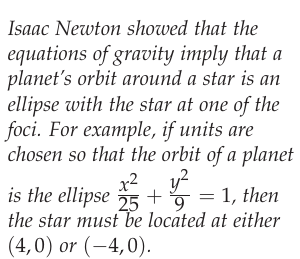
\includegraphics[scale=0.5]{ellipse1.png}
  \end{figure}
 \end{frame}

 \begin{frame}
  \frametitle{Ellispe}
  \begin{figure}
    \centering
    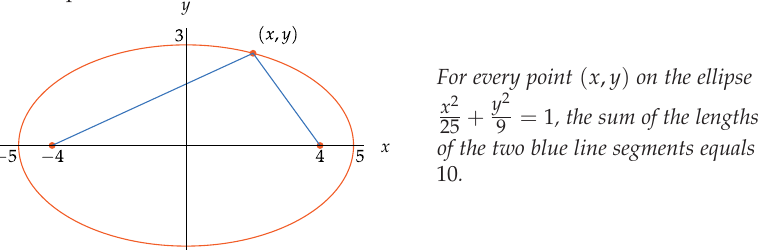
\includegraphics[scale=0.4]{foci.png}
  \end{figure}
 \end{frame}

 \begin{frame}{Eccentricity of an Ellipse}
  \begin{block}{Definition}
      The \textbf{eccentricity} ($e$) of an ellipse is a measure of how much the ellipse deviates from being a circle. It is defined as
      \[
      e = \frac{c}{a} .
      \]
      \[
  c^2 = a^2 - b^2,
  \]
  \[e = \sqrt{1 - \frac{b^2}{a^2}}\]
      where:
      \begin{itemize}
          \item $c$ is the distance from the center to a focus.
          \item $a$ is the length of the semi-major axis.
      \end{itemize}
  \end{block}
  
  
 
\end{frame}

\begin{frame}
  \frametitle{Eccentricity}
  \bigskip
  \begin{center}
  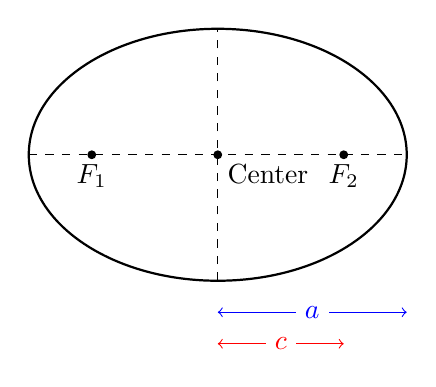
\begin{tikzpicture}[scale=0.8]
      % Draw the ellipse
      \draw[thick] (0,0) ellipse (3cm and 2cm);
      
      % Draw major and minor axes
      \draw[dashed] (-3,0) -- (3,0);
      \draw[dashed] (0,-2) -- (0,2);
      
      % Mark the center
      \fill (0,0) circle (2pt) node[below right] {Center};
      
      % Mark the foci
      \fill (-2,0) circle (2pt) node[below] {$F_1$};
      \fill (2,0) circle (2pt) node[below] {$F_2$};
      
      % Indicate the semi-major axis (a)
      \draw[<->, blue] (0, -2.5) -- (3, -2.5) node[midway, fill=white] {$a$};
      
      % Indicate the focal distance (c)
      \draw[<->, red] (0, -3.0) -- (2, -3.0) node[midway, fill=white] {$c$};
  \end{tikzpicture}
  \end{center}
  Additionally, the semi-minor axis $b$ is related to $a$ and $c$ by:
  
  \bigskip
  \textbf{Key Points:}
  \begin{itemize}
      \item If $e = 0$, the ellipse is a circle.
      \item If $0 < e < 1$, the ellipse is elongated, with greater elongation as $e$ increases.
  \end{itemize}
\end{frame}

\begin{frame}
  \frametitle{Hyperbola}
\begin{block}{Definition}
  The graph of the equation of the form 
  \[
\frac{y^2}{b^2} - \frac{x^2}{a^2} = 1
\]
where \(a,b\) are non-zero numbers
\end{block}
\end{frame}

\begin{frame}
  \begin{figure}
    \centering 
    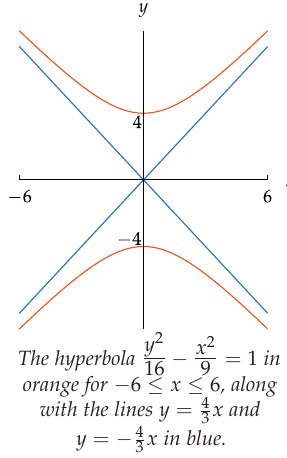
\includegraphics[scale=0.5]{hyperbola2.png}
  \end{figure}
\end{frame}
\begin{frame}
  \frametitle{Hyperbola}
  \begin{block}{Foci}
    The foci of a hyperbola are two points with the property that the difference of
the distances from the foci to a point on the hyperbola is a constant independent
of the point on the hyperbola
  \end{block}
\end{frame}

\begin{frame}
  \begin{figure}
    \centering 
    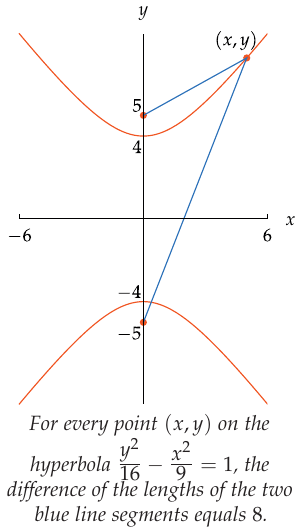
\includegraphics[scale=0.4]{hyperbola3.png}
  \end{figure}
\end{frame}
\begin{frame}
  \begin{figure}
    \centering 
    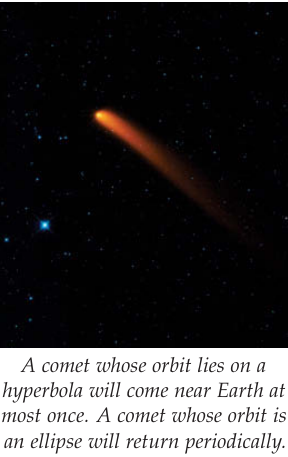
\includegraphics[scale=0.5]{hyperbola1.png}
  \end{figure}
\end{frame}

\subsection{Exponents}
\begin{frame}
  \frametitle{Positive Integer Exponent}
  \begin{block}{Positive Integer Exponent}
    If \(x\) is a real number and \(m\) is a positive integer, then \(x^{m}\) is defined to be the
product with \(x\) appearing \(m\) times
\[x^{m} = \underset{x \;\;appears\;\;m \;\;times}{\underbrace{x \cdot x \cdots x }}\]
    
  \end{block}
\end{frame}

\begin{frame}
  \frametitle{Positive Integer Exponenets}
  \begin{block}{Properties}
    Suppose \(x\) and \(y\) are numbers and \(m\) and \(n\) are positive integers. Then 
    \[x^{m}x^{n} = x^{m+n} \]   
    \[\left(x^{m}\right)^{n} = x^{mn} \] 
    \[x^{m}y^{m} = \left(xy\right)^{m} \] 
  \end{block}
\end{frame}
\begin{frame}
  \frametitle{\(x^{0}\)} 
  \begin{alertblock}{What is \(x^{0}\)}
    If  \(x^{m}x^{n} = x^{m+n}\) then we can write \[x^{0}x^{n} = x^{0+n} = x^{n} \implies x^{0} = 1\;for\;\ x \neq 0\]
   \end{alertblock}

   \begin{alertblock}{What is \(0^{0}\)}
    \begin{itemize}
      \item The rule \( x^0 = 1 \) (for \( x \neq 0 \)) suggests that \( 0^0 \) should be \(1\).
      \item The rule \( 0^m = 0 \) (for \( m > 0 \)) suggests that \( 0^0 \) should be \(0\)
      \item Since these two rules contradict each other, \( 0^0 \) is left undefined in general mathematics.
      \item However, in combinatorics and programming, \( 0^0 \) is often defined as \(1\) for convenience.
  \end{itemize}
   \end{alertblock}
\end{frame}

\begin{frame}
  \frametitle{Negative Integer Exponents}
  If \(x^{m}x^{n} = x^{m+n}\), if we take \(m = -n \), then 
  \[x^{m}x^{-m} = x^{0} = 1 \implies x^{m}x^{-m} = 1\]
  We have to define \(x^{-m}\) to equal the multiplicative inverse of \(x^{m}\)
\begin{block}{Negative Interger Exponent}
  If \(x \neq 0\) and \(m\) is a positive integer, then \(x^{-m}\) is defined to multiplicative inverse of \(x^{m}\) 
  \[x^{-m} = \frac{1}{x^{m}}\]
  
\end{block}
\end{frame}
\begin{frame}
  \frametitle{Exponents: Some Graphs}
  
  

  

\end{frame}
\end{document}